\documentclass[../main.tex]{subfiles}

\begin{document}
\section{Results}\label{sec:results}
We will here present the results of our simulations. In all simulations done, a fixed set of parameter values were used unless stated otherwise. Those values are described in \cref{sec:populations}.

\iffalse
\begin{table}[!htb]
\centering
\label{tb:param}
\begin{tabular}{|c|l|l|l|l|l|}
\hline
Parameter & \multicolumn{1}{c|}{$S_0$} & \multicolumn{1}{c|}{$I_0$} & \multicolumn{1}{c|}{$R_0$} & \multicolumn{1}{c|}{$a$} & \multicolumn{1}{c|}{$c$} \\ \hline
Value & 300 & 100 & 0.0 & 4 & 0.5 \\ \hline
\end{tabular}
\caption{The set of parameters that stayed constant during simulations.}
\end{table}
\fi

\subsection{Simple SIRS model}
As explained in \cref{sec:populations}, we want to see how a disease spreads in four identical populations when the only parameter that changes is the rate of recovery $b$ of the disease. The results can be seen in figure (\ref{fig:mc:base}), where we compare both a simulation based on the Runge Kutta 4th order method and a method using Monte Carlo simulation. 

\iffalse
In \cref{fig:SIRS_rk4}, the temporal variations of the number of individuals for the three classes ($S$, $I$, $R$) are compared for $b=1$, 2, 3, 4 using the fourth-order Runge-Kutta method. Here, the other parameters are fixed as explained in \cref{sec:populations}. 
\fi

\iffalse
\begin{figure}[htb!]
    \centering
    \begin{subfigure}[b]{0.475\textwidth}
    \centering
    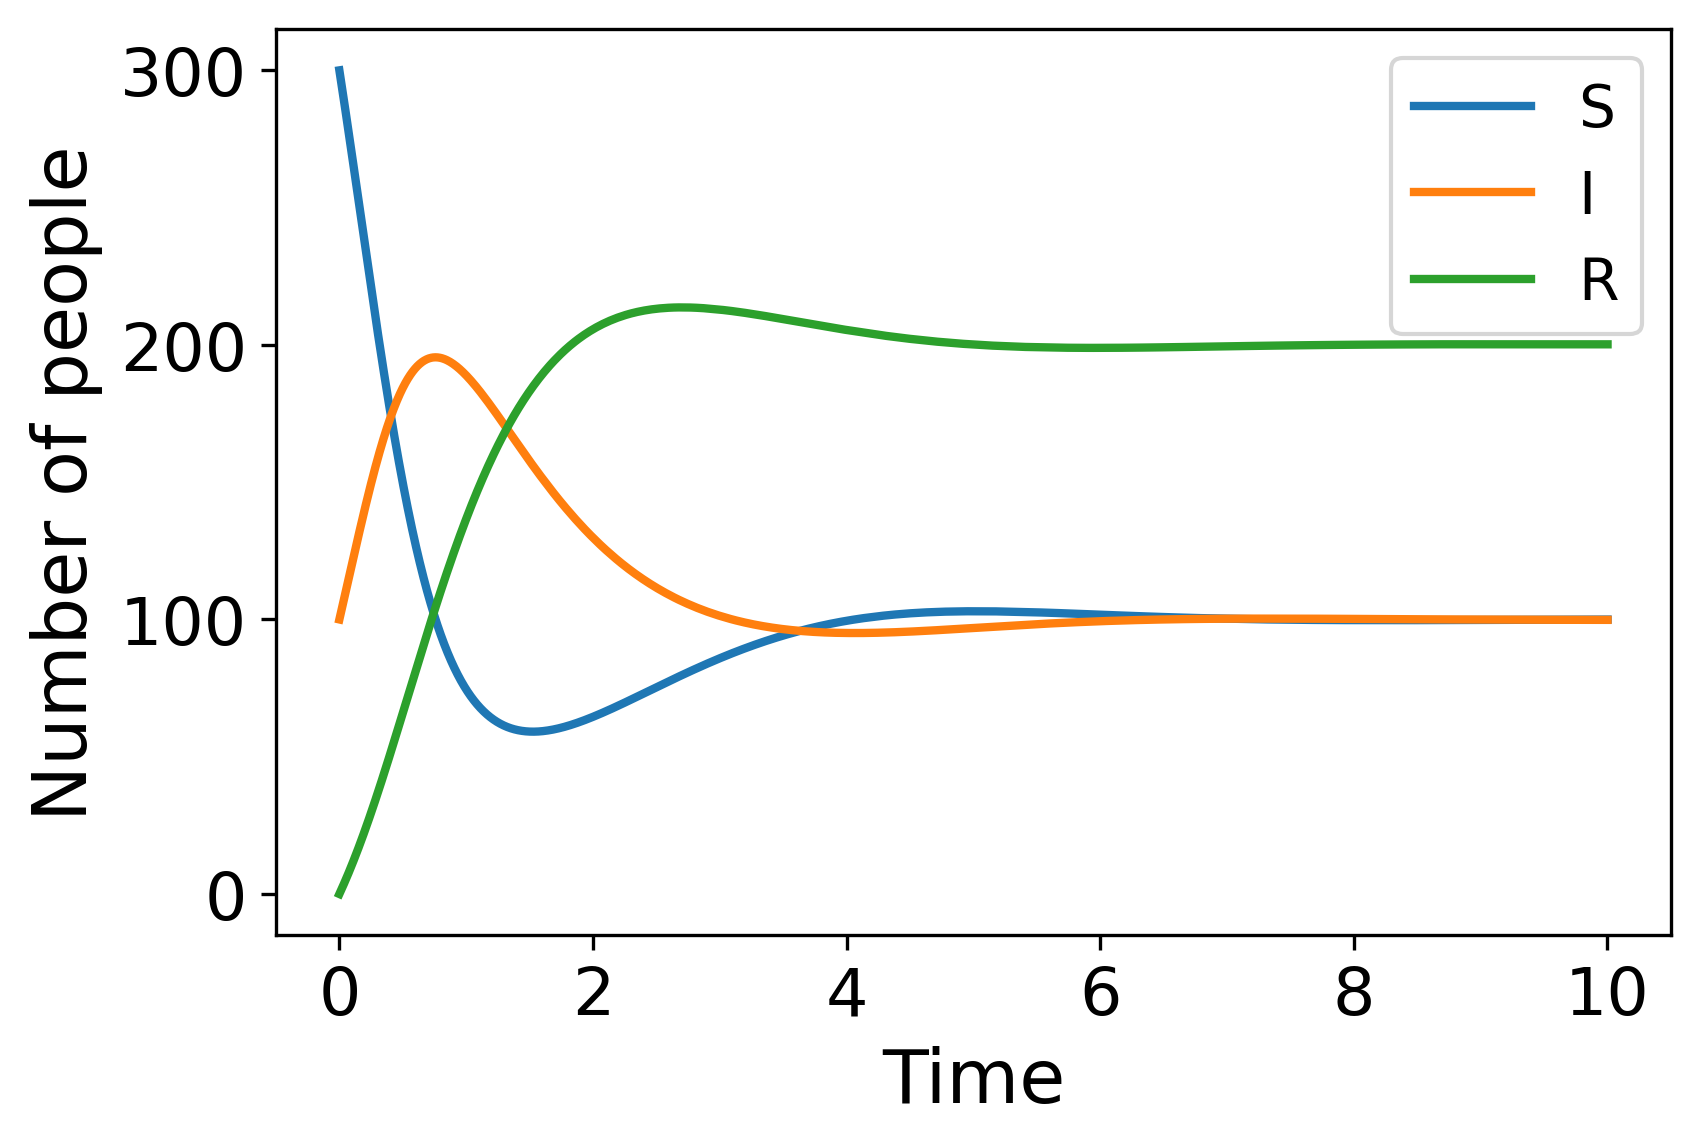
\includegraphics[width=0.9\textwidth]{../figures/SIRS_rk4_b=1.png}
    \caption{}
    \label{fig:b=1}
    \end{subfigure}
    \quad
    \begin{subfigure}[b]{0.475\textwidth}
    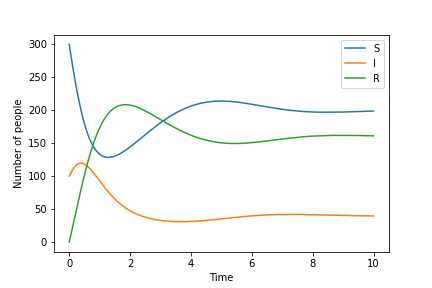
\includegraphics[width=0.9\textwidth]{../figures/SIRS_rk4_b=2.png}
    \caption{}
    \label{fig:b=2}
    \end{subfigure}
    
    \begin{subfigure}[b]{0.475\textwidth}
    \centering
    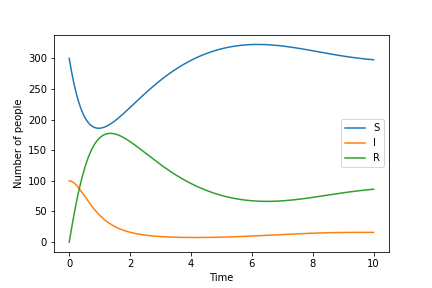
\includegraphics[width=0.9\textwidth]{../figures/SIRS_rk4_b=3.png}
    \caption{}
    \label{fig:b=3}
    \end{subfigure}
    \quad
    \begin{subfigure}[b]{0.475\textwidth}
    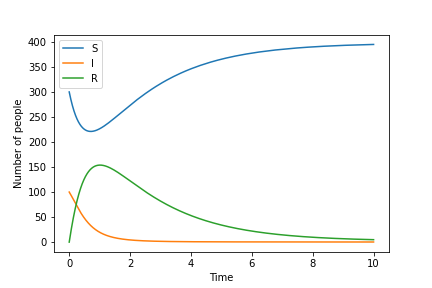
\includegraphics[width=0.9\textwidth]{../figures/SIRS_rk4_b=4.png}
    \caption{}
    \label{fig:b=4}
    \end{subfigure}
    \caption{The numerical solution of the SIRS model using the fourth-order Runge-Kutta method with $N=400$, $I(0)=100$, $a=4$, $c=0.5$ fixed and the comparison of $S$, $I$, $R$ for (a)  $b=1$, (b) $b=2$, (c) $b=3$ and (d) $b=4$.}
    \label{fig:SIRS_rk4}
\end{figure}
\fi


\begin{figure}[!htb]
\centering
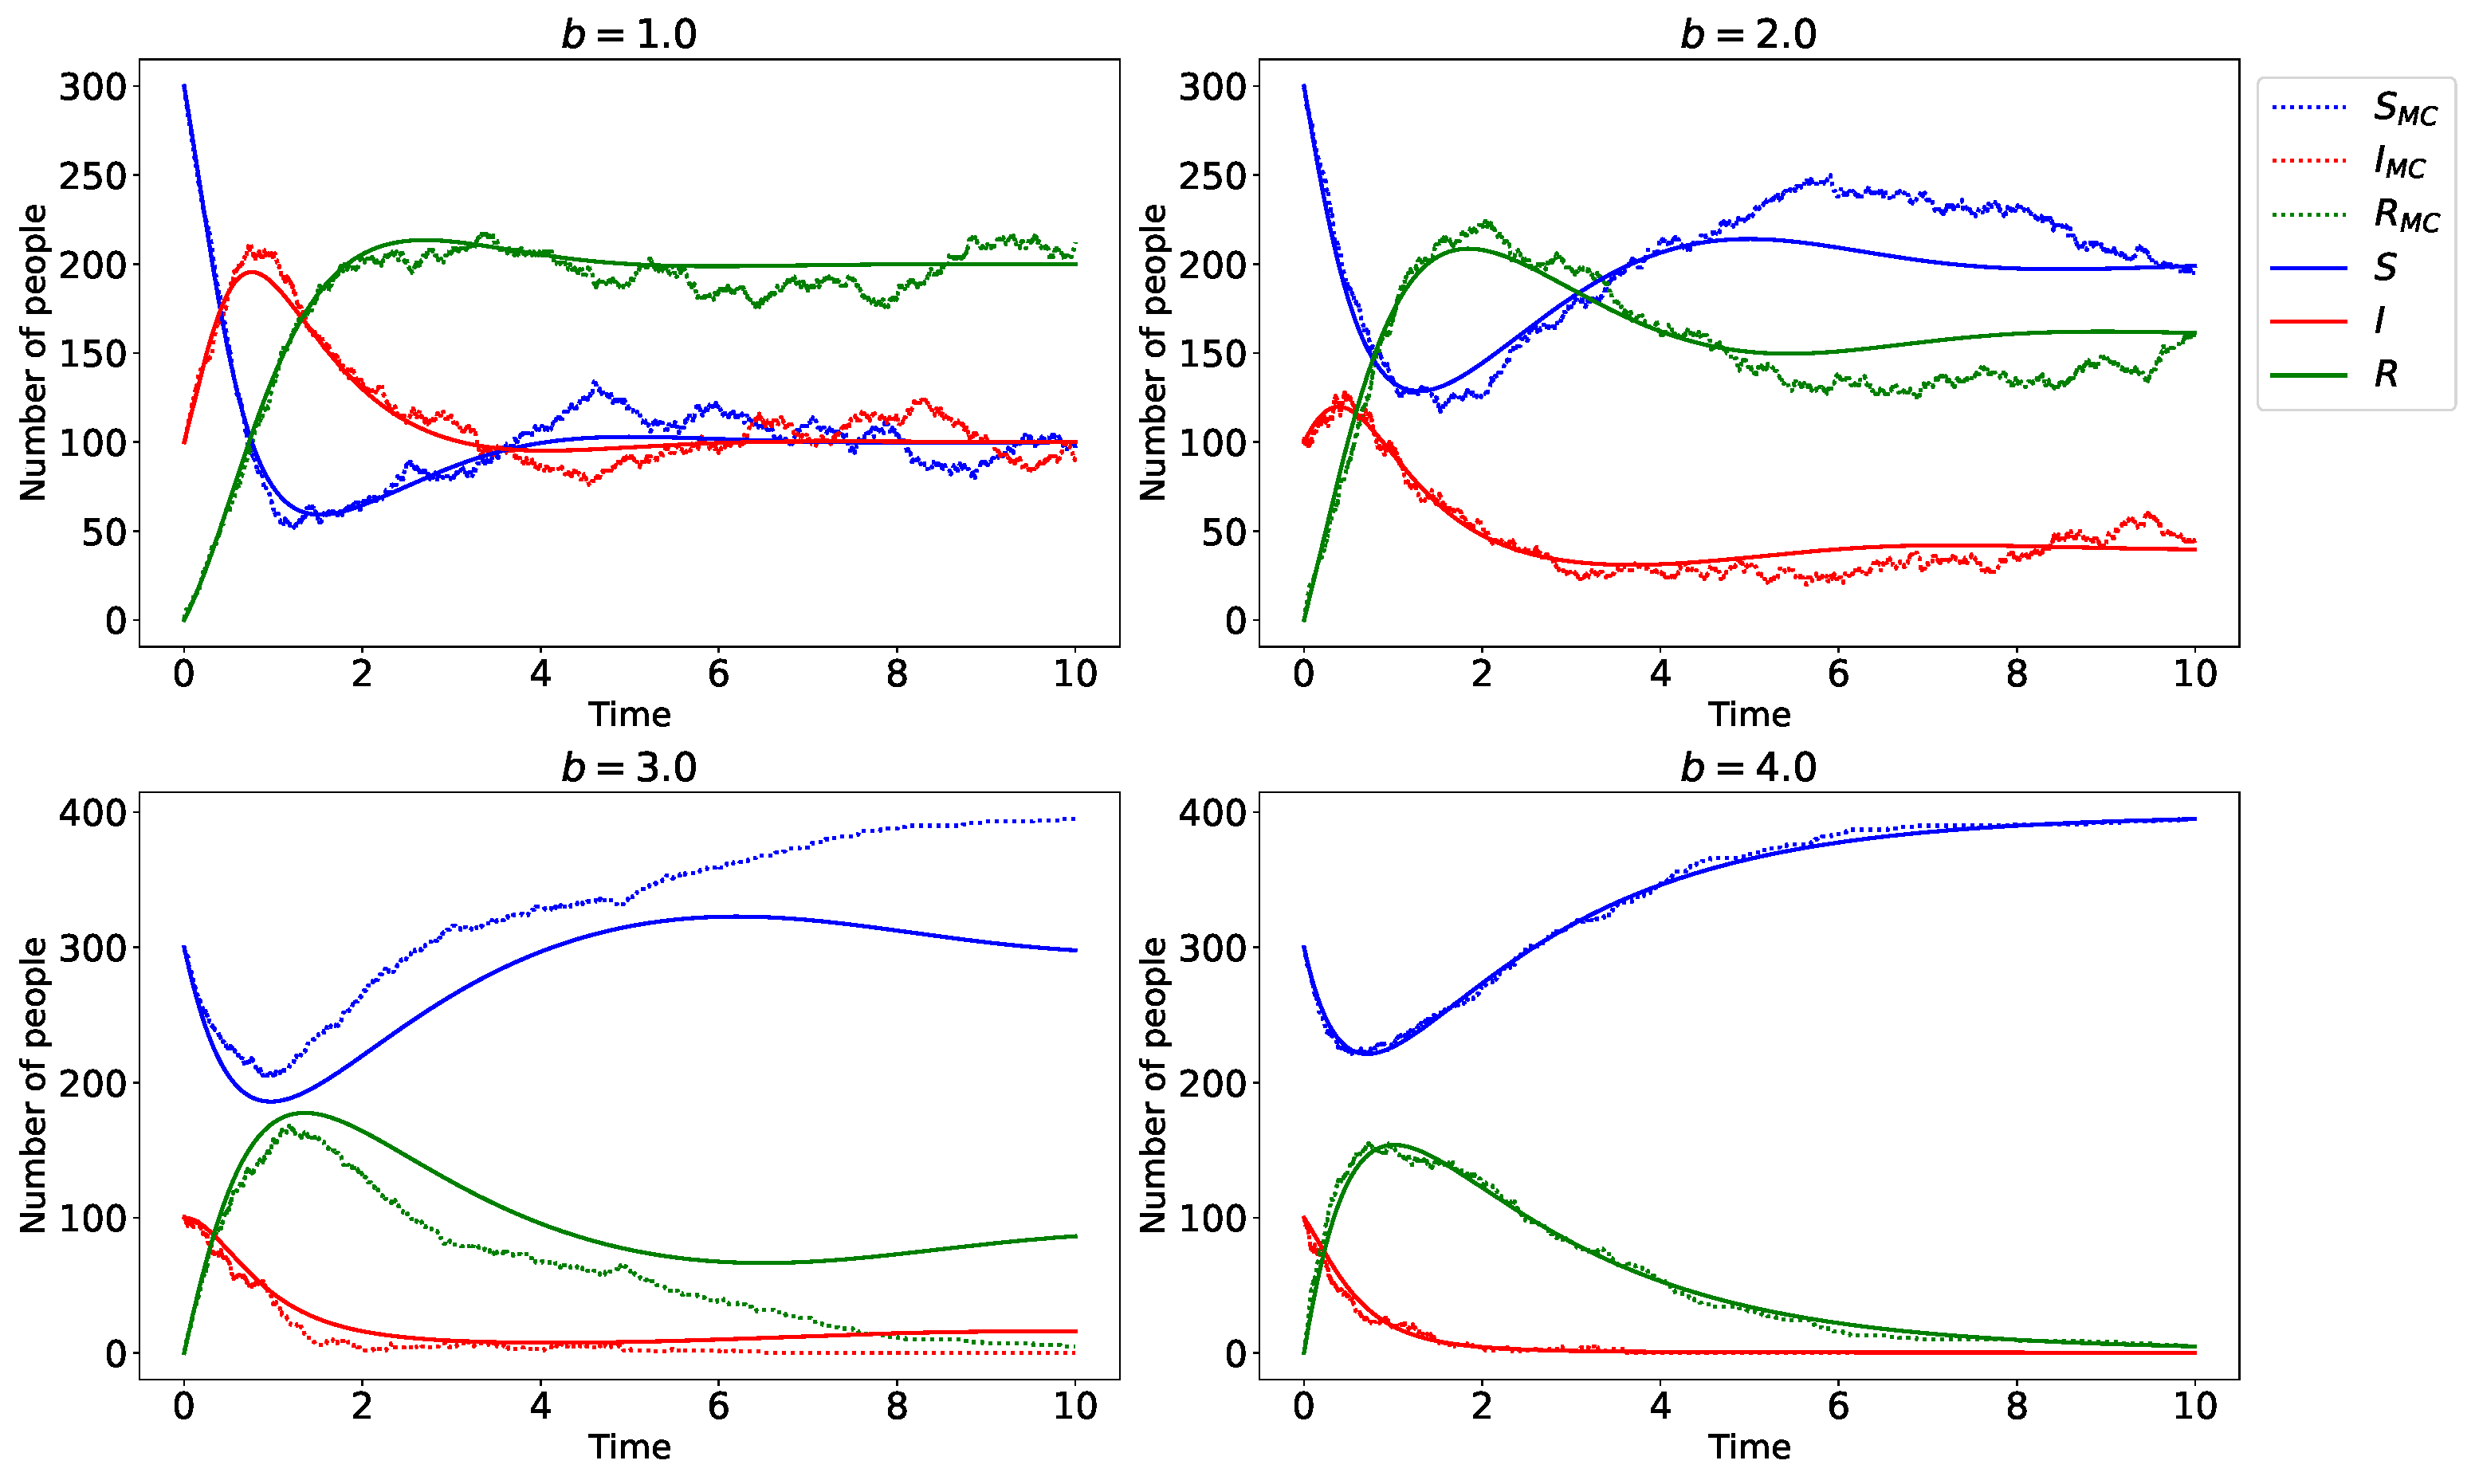
\includegraphics[width=\textwidth]{../figures/rk4_vs_mc_base.pdf}
\caption{Monte Carlo  and RK4 simulation of base SIRS model for varying $b$ values.}
\label{fig:mc:base}
\end{figure}

\newpage
\iffalse
For $b=1$, as seen in \cref{fig:b=1}, the number of susceptible individuals decreases with time, reaches a minimum of 59 individuals, gradually increases and reaches an equilibrium at 100 susceptible individuals.
The number of infected individuals increases with time, reaches a peak of 195, gradually decreases and reaches an equilibrium of 100 infected individuals. Meanwhile, the number of recovered individuals increases gradually, has a small dip and reaches an equilibrium at 200 recovered individuals. Next, we look at $b=2$, as seen in \cref{fig:b=2}. Here, the the number of susceptible individuals decreases with time, reaches a minimum of 128 individuals, gradually increases and reaches an equilibrium of 199 susceptible individuals. The number of infected individuals increases for a brief period of  time, reaches a peak of 120, gradually decreases and reaches an equilibrium of 40 infected individuals. While the number of recovered individuals increases gradually, has a small dip and reaches an equilibrium of 161 recovered individuals.
Turning now to  $b=3$, as seen in \cref{fig:b=3}. The number of susceptible individuals gradually decreases with time, reaches a minimum of 185 and approaches 208 with time. The number of infected individuals gradually decreases and approaches 16 with time. The number of recovered individuals increases, reaches a peak of 177 and gradually approaches 86.
Finally, we look at $b=4$ in \cref{fig:b=4}. As expected, the disease does not establish itself in the population. The number of infected individuals gradually decreases and approaches zero with time. While the number of recovered individuals increases, reaches a peak of 154 and gradually approaches zero. 
\fi

\iffalse
\begin{figure}[htb]
\centering
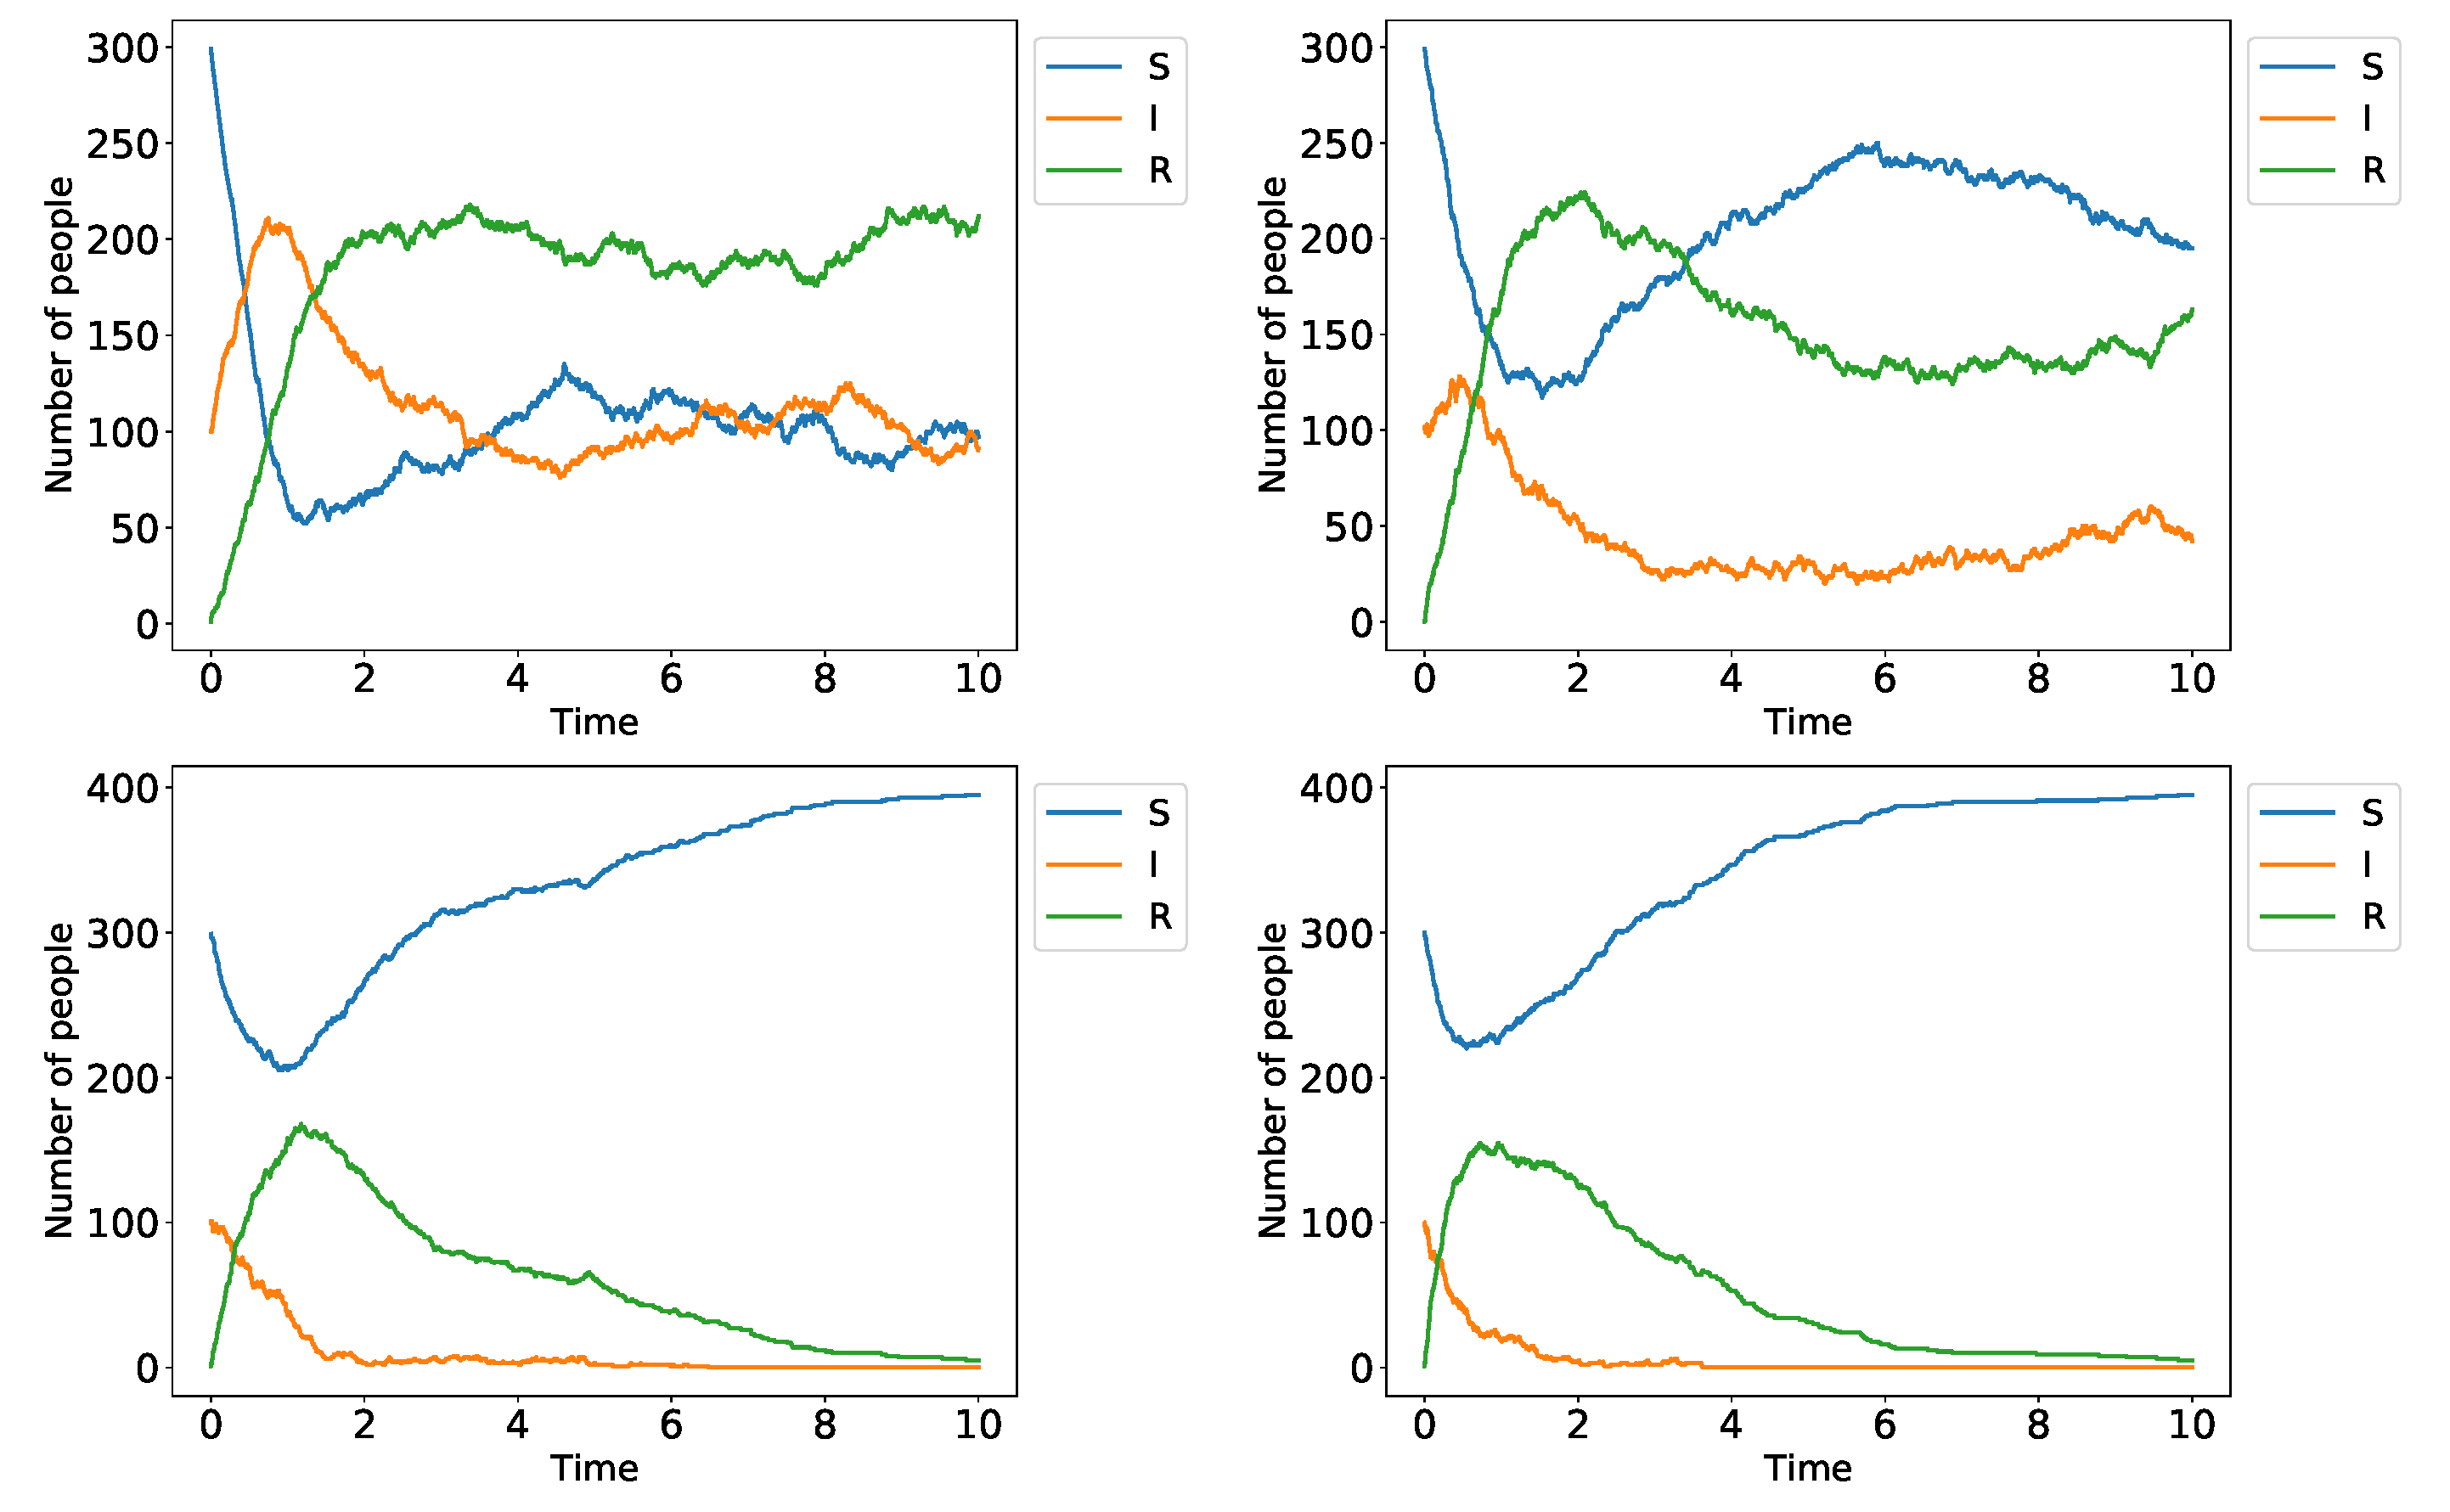
\includegraphics[width=\textwidth]{../figures/MC_a.pdf}
\caption{Monte Carlo simulation of base SIRS model for varying $b$ values. Initial values are $S_0 = 300$, $I_0 = 100$, $a = 4$ and $c = 0.5$}
\label{fig:mc:base}
\end{figure}
\fi


\begin{figure}[!htb]
\centering
\includegraphics[width=\textwidth]{../figures/RK4_vs_MC.pdf}
\caption{A closer look at the results of RK4 and MC for a sample population with $b = 1$. Also shown is the standard deviation $\sigma$ over several simulations using the MC method and the corresponding expectation values $E$.}
\label{fig:mc:comparison}
\end{figure}



\subsection{SIRS model with vital dynamics}
We know want to look at what would happen to a sample population where vital dynamics have been added. In this case, we wish to see how the deadliness of the disease impacts the population as a whole. 


\iffalse
\Cref{fig:SIRS_rk4_vital} displays the temporal variations of the number of individuals for the three classes ($S$, $I$, $R$) which are compared for $b=1$, 2, 3, 4 using the fourth-order Runge-Kutta method. 

\begin{figure}[htb!]
    \centering
    \begin{subfigure}[b]{0.475\textwidth}
    \centering
    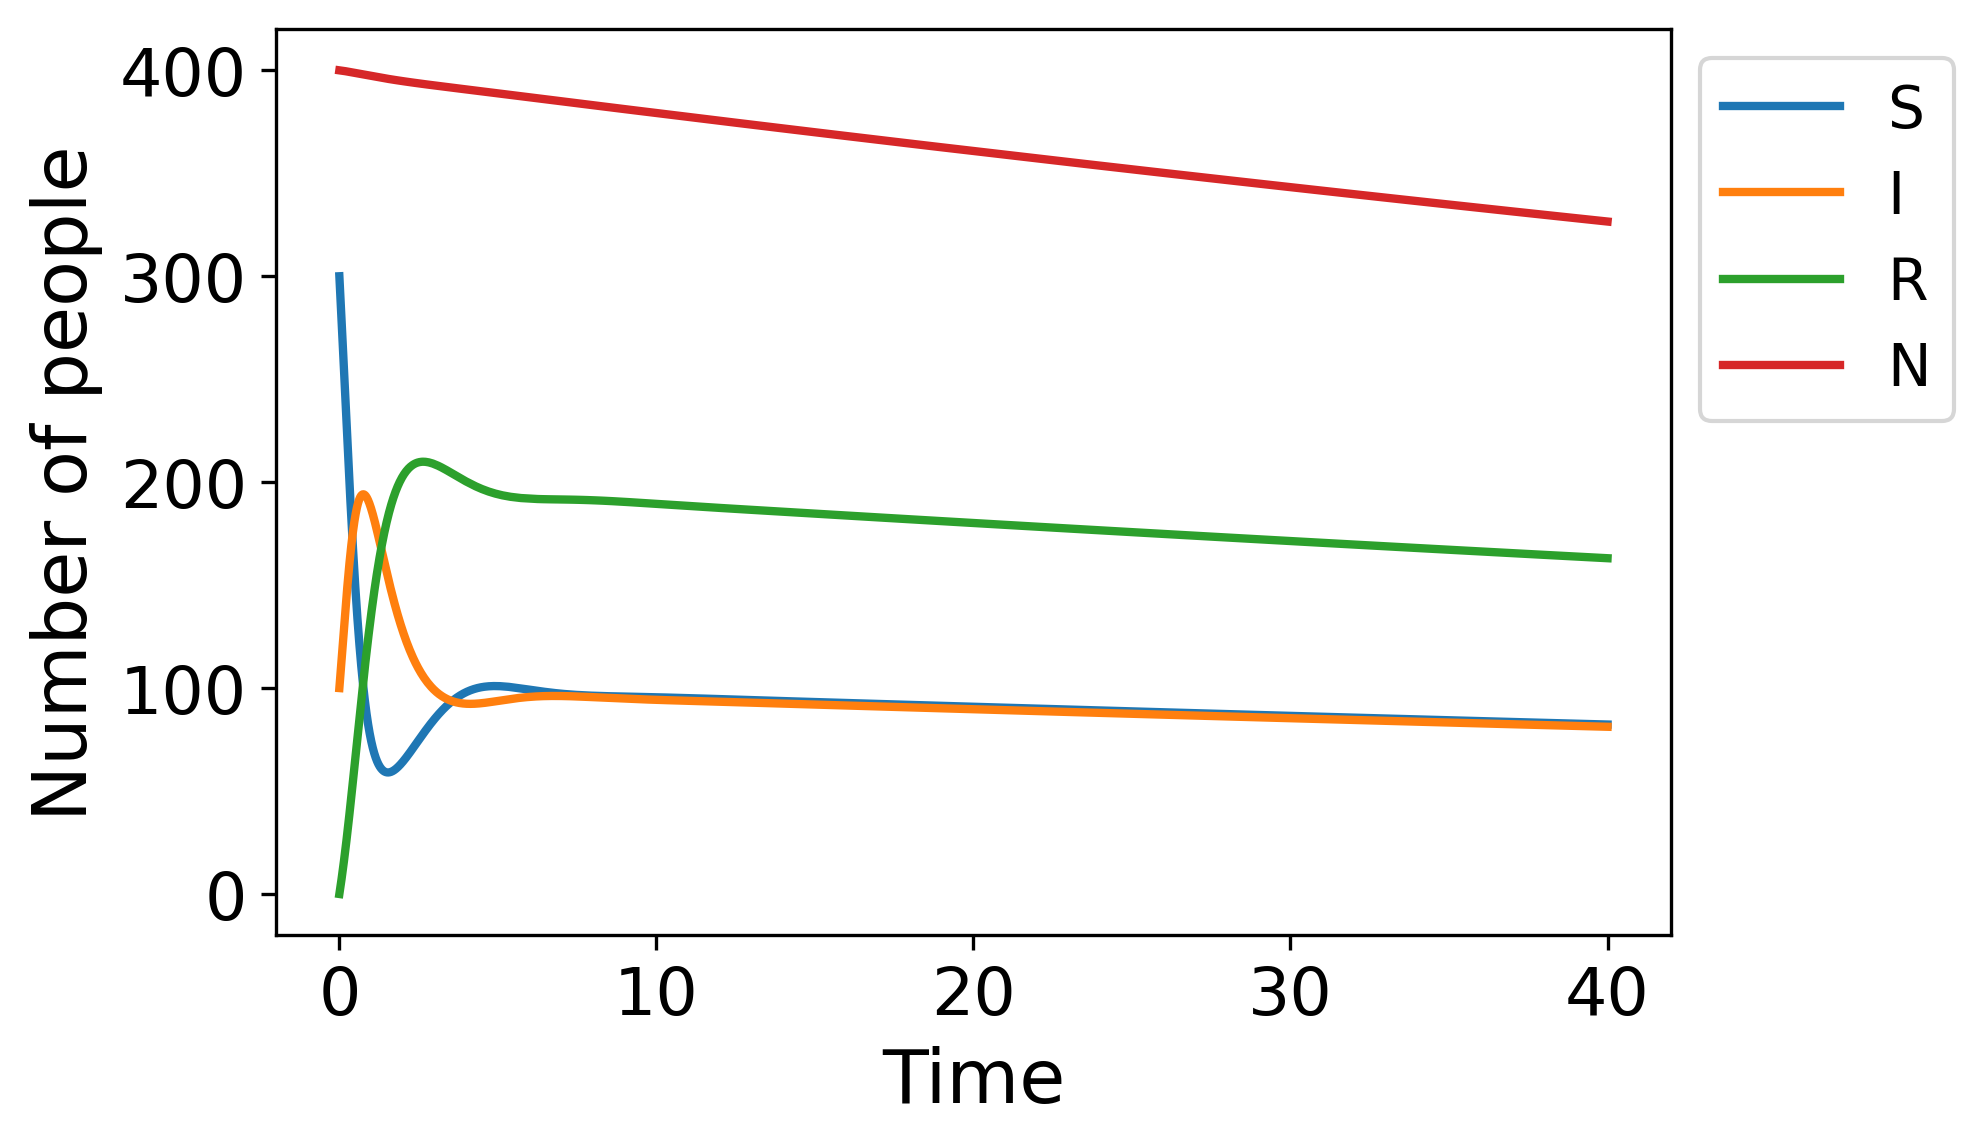
\includegraphics[width=0.9\textwidth]{../figures/SIRS_vital_rk4_b=1.png}
    \caption{}
    \label{fig:vital_b=1}
    \end{subfigure}
    \quad
    \begin{subfigure}[b]{0.475\textwidth}
    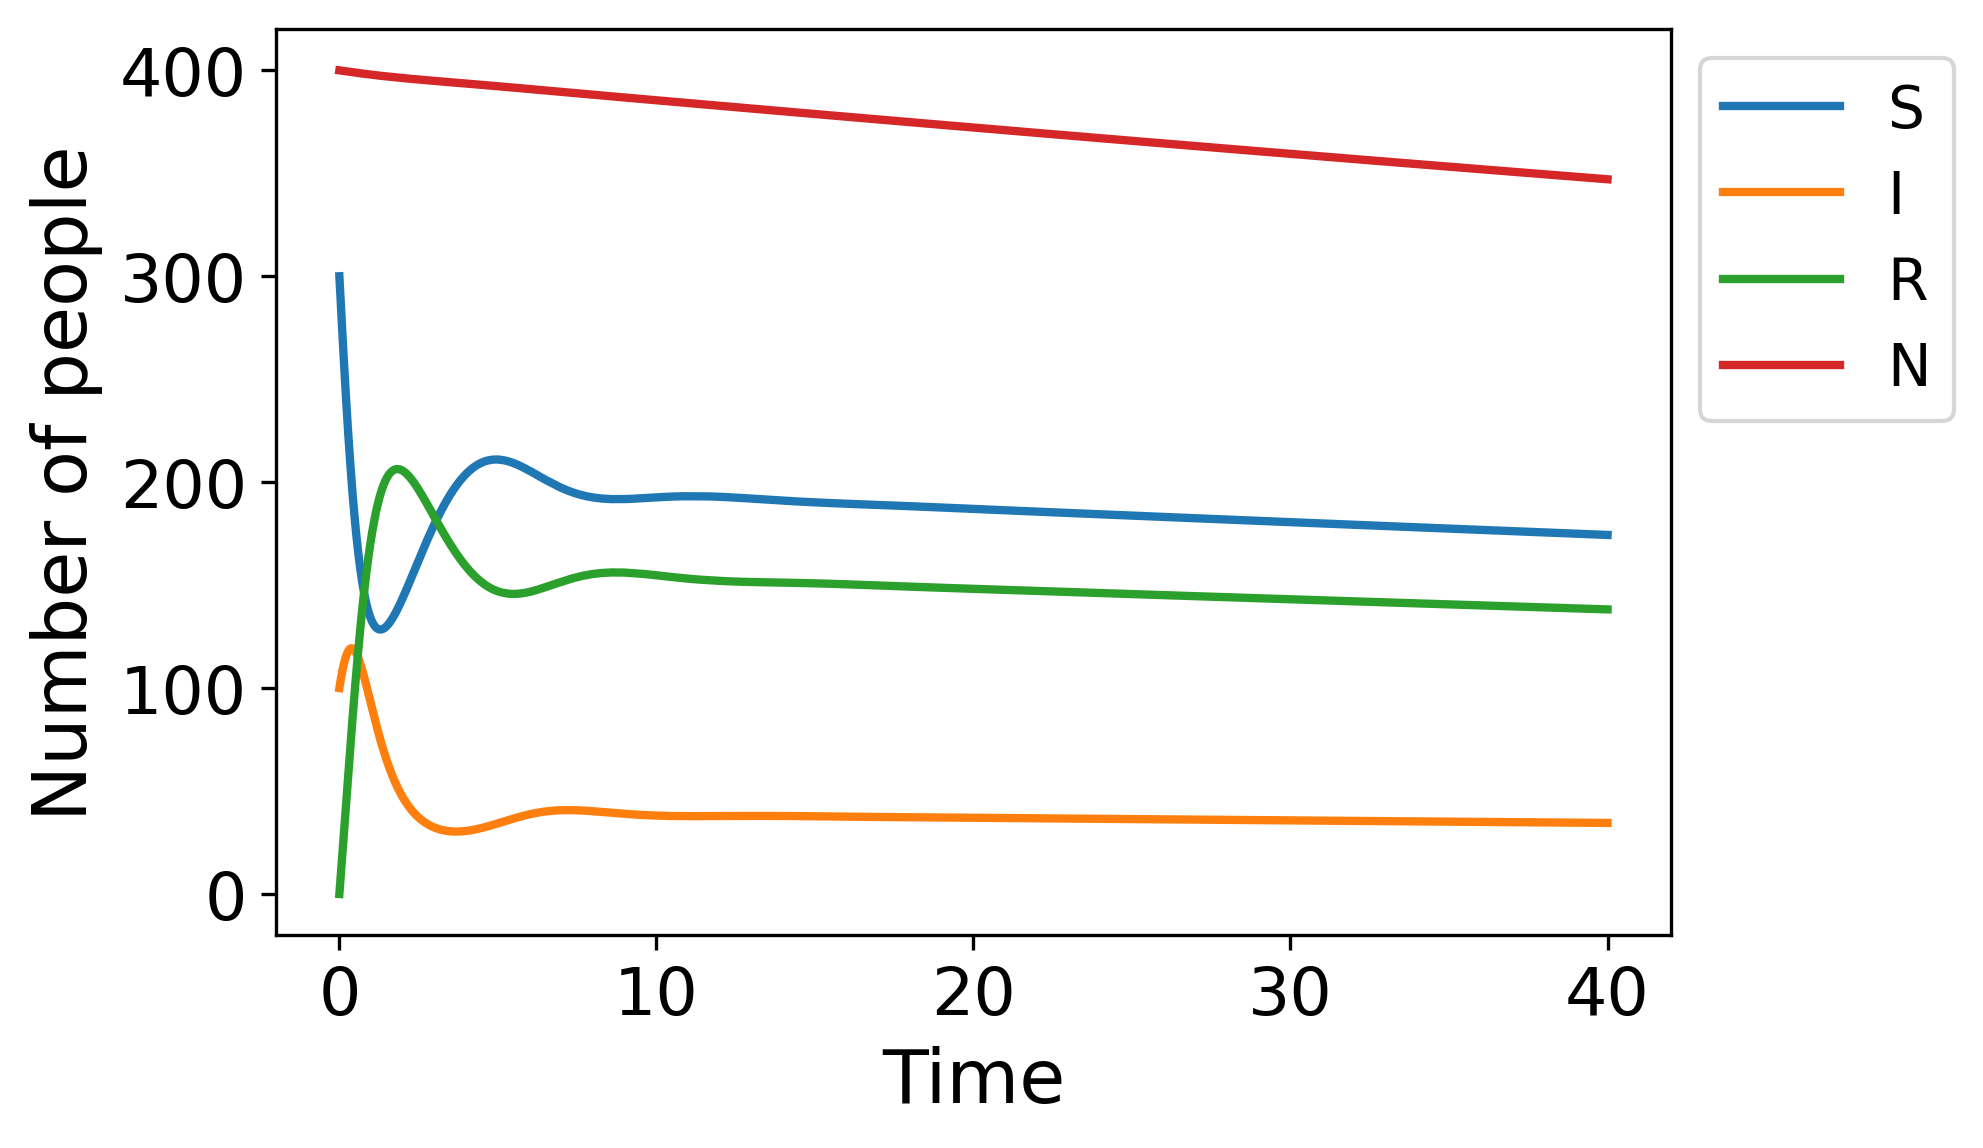
\includegraphics[width=0.9\textwidth]{../figures/SIRS_vital_rk4_b=2.png}
    \caption{}
    \label{fig:vital_b=2}
    \end{subfigure}
    
    \begin{subfigure}[b]{0.475\textwidth}
    \centering
    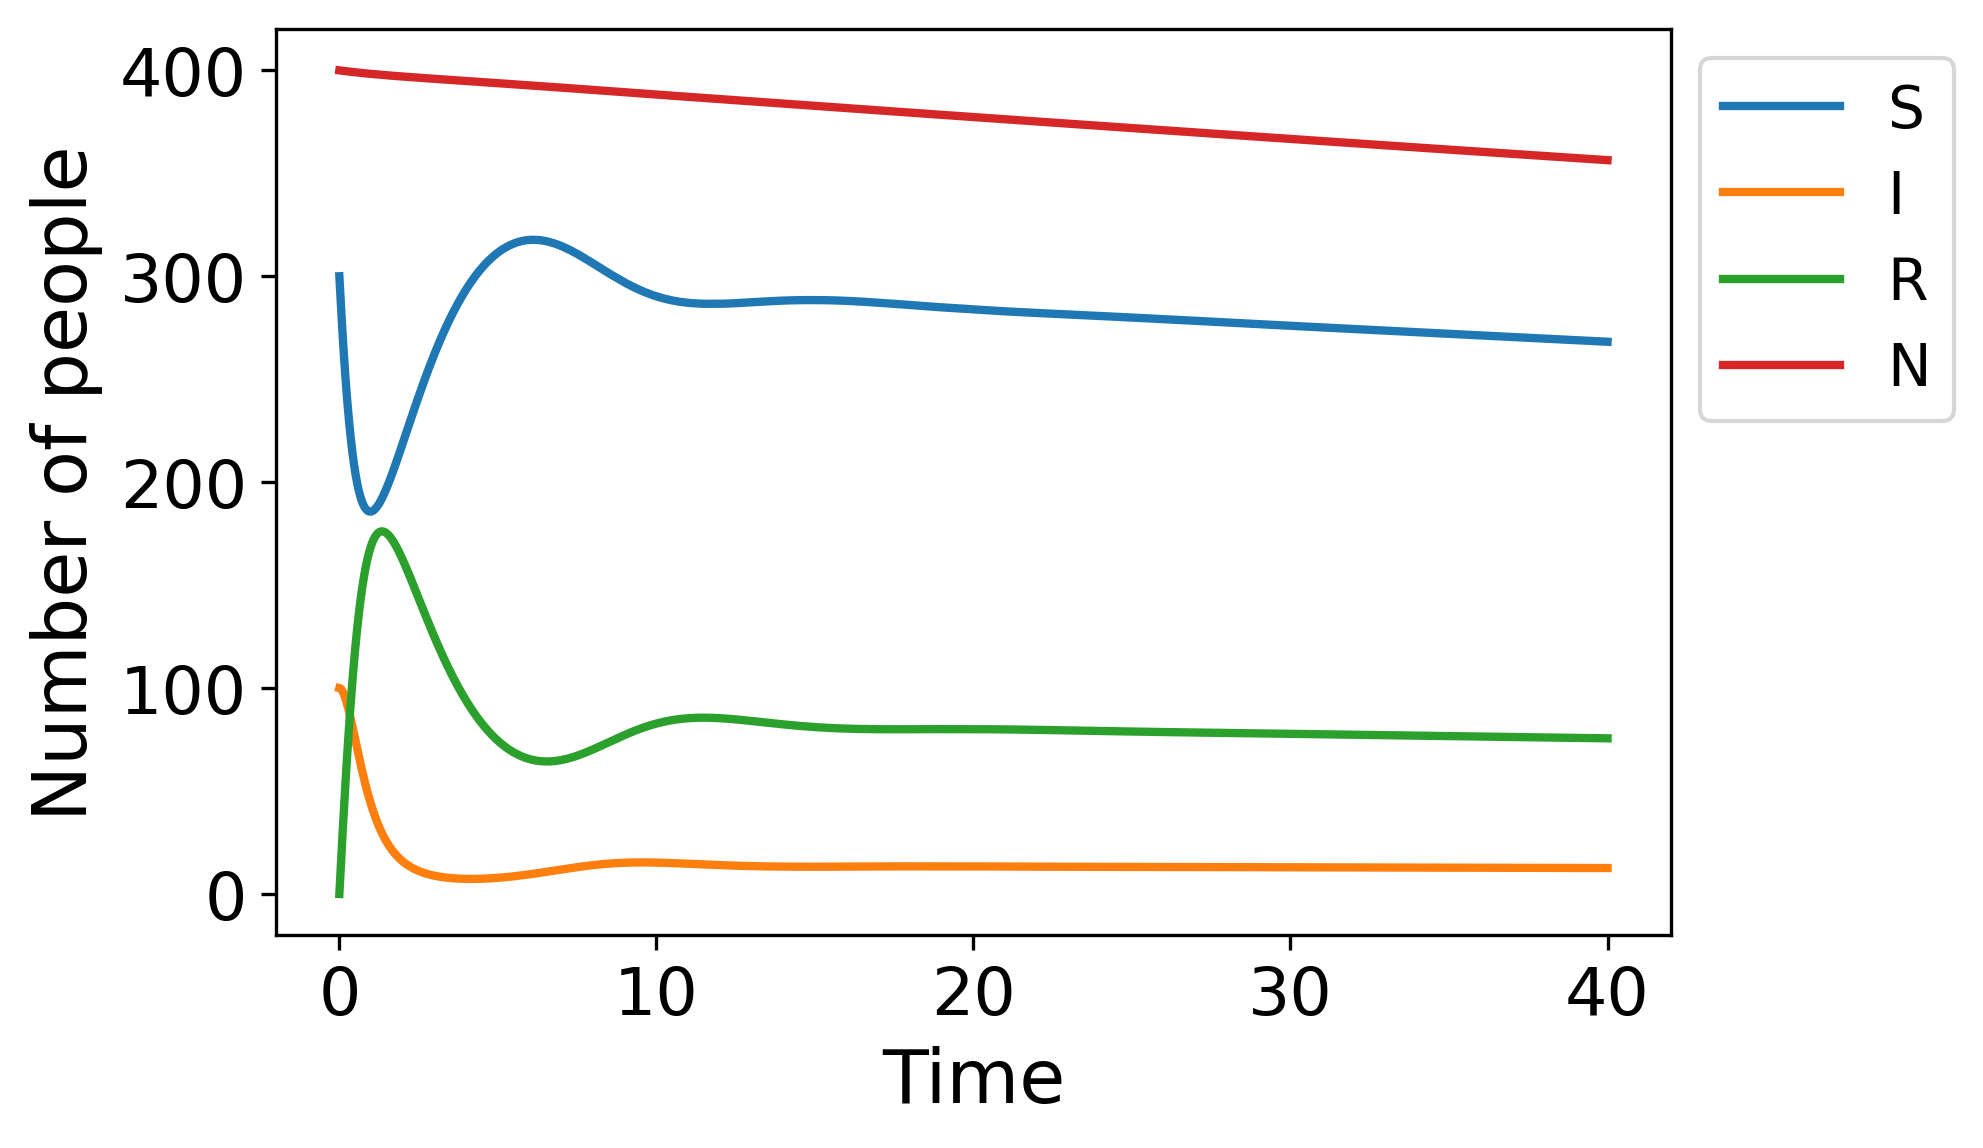
\includegraphics[width=0.9\textwidth]{../figures/SIRS_vital_rk4_b=3.png}
    \caption{}
    \label{fig:vital_b=3}
    \end{subfigure}
    \quad
    \begin{subfigure}[b]{0.475\textwidth}
    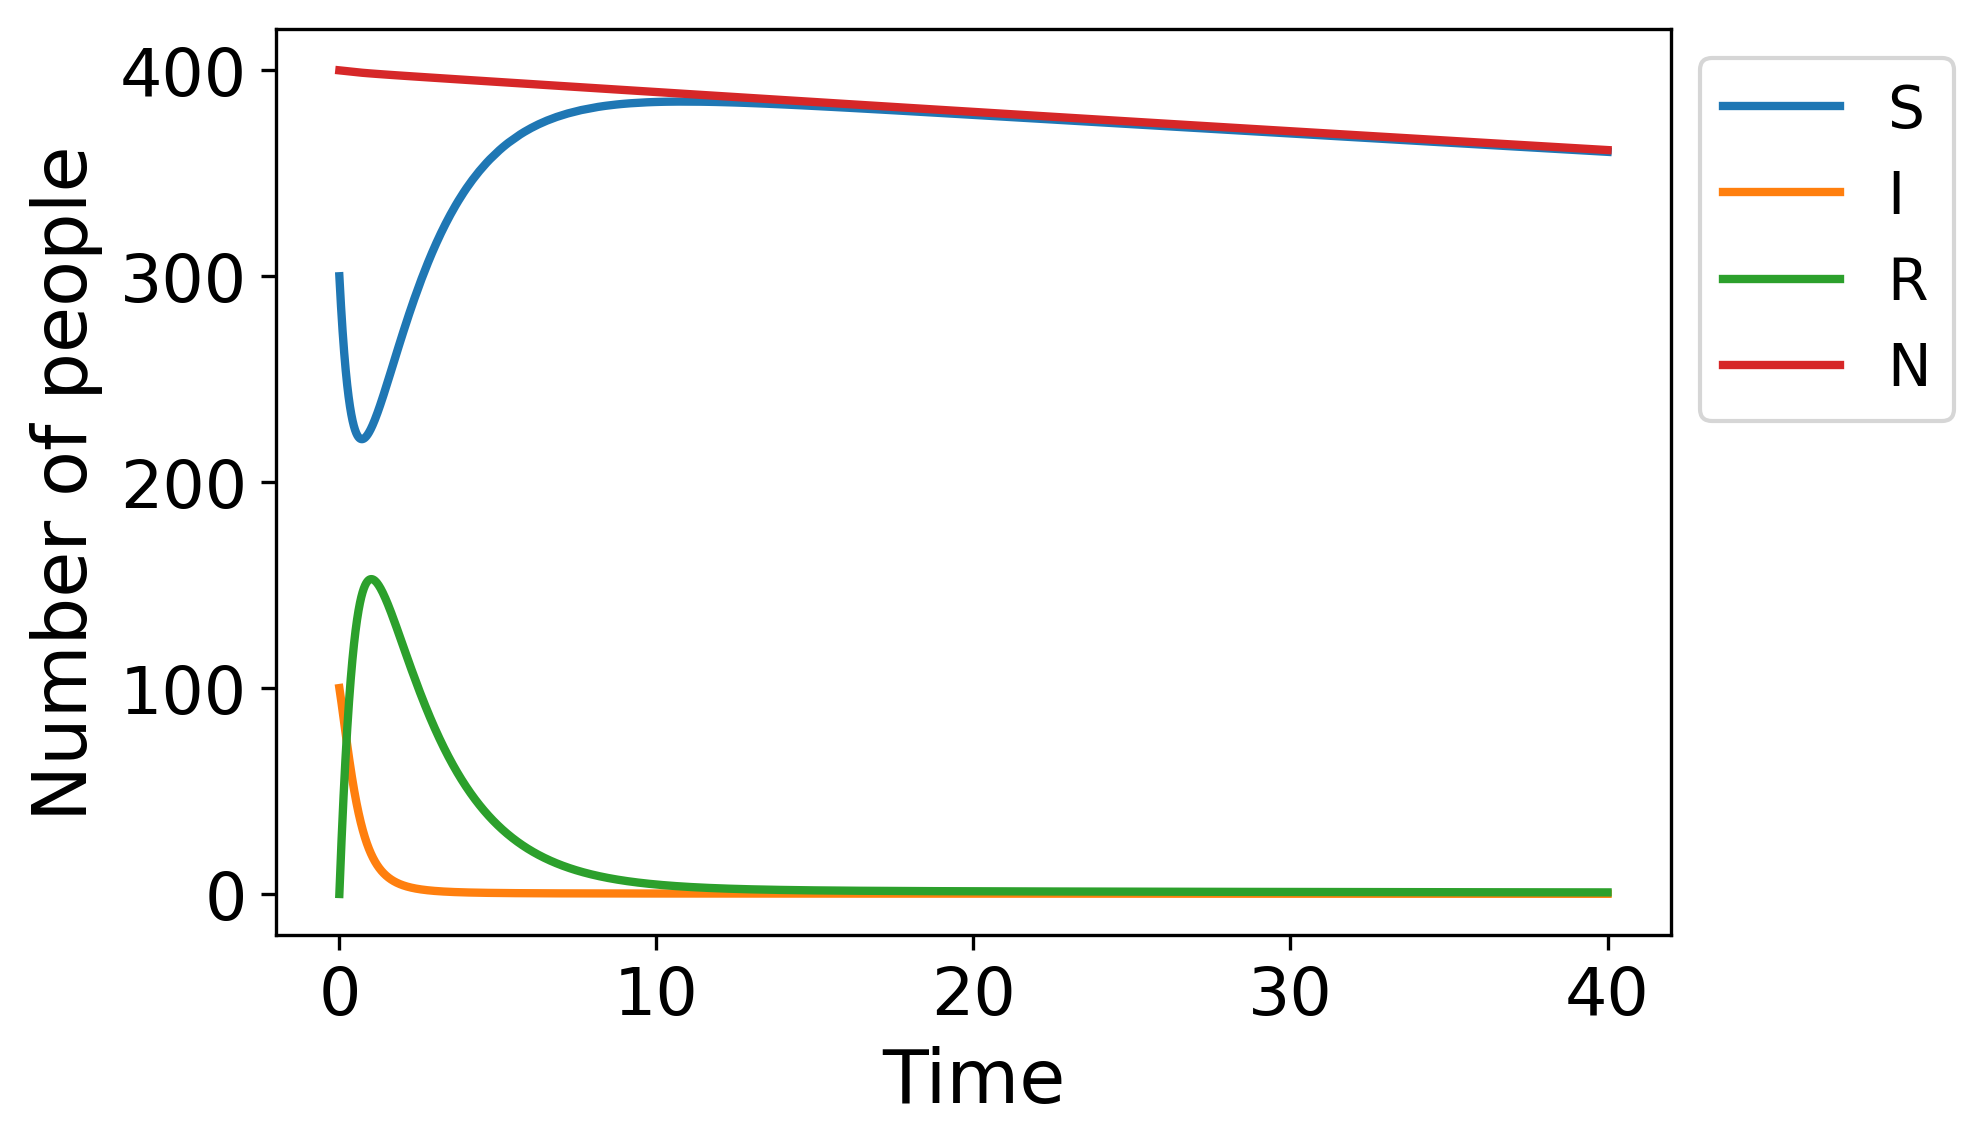
\includegraphics[width=0.9\textwidth]{../figures/SIRS_vital_rk4_b=4.png}
    \caption{}
    \label{fig:vital_b=4}
    \end{subfigure}
    \caption{The numerical solution of the SIRS model with vital dynamics using the fourth-order Runge-Kutta method with $N(0)=400$, $I(0)=100$, $a=4$, $c=0.5$, $d=0.0003$, $d_I=0.01$, $e=0.0005$ fixed and the comparison of $S$, $I$, $R$ for (a)  $b=1$, (b) $b=2$, (c) $b=3$ and (d) $b=4$.}
    \label{fig:SIRS_rk4_vital}
\end{figure}
\fi


\begin{figure}[!htb]
\centering
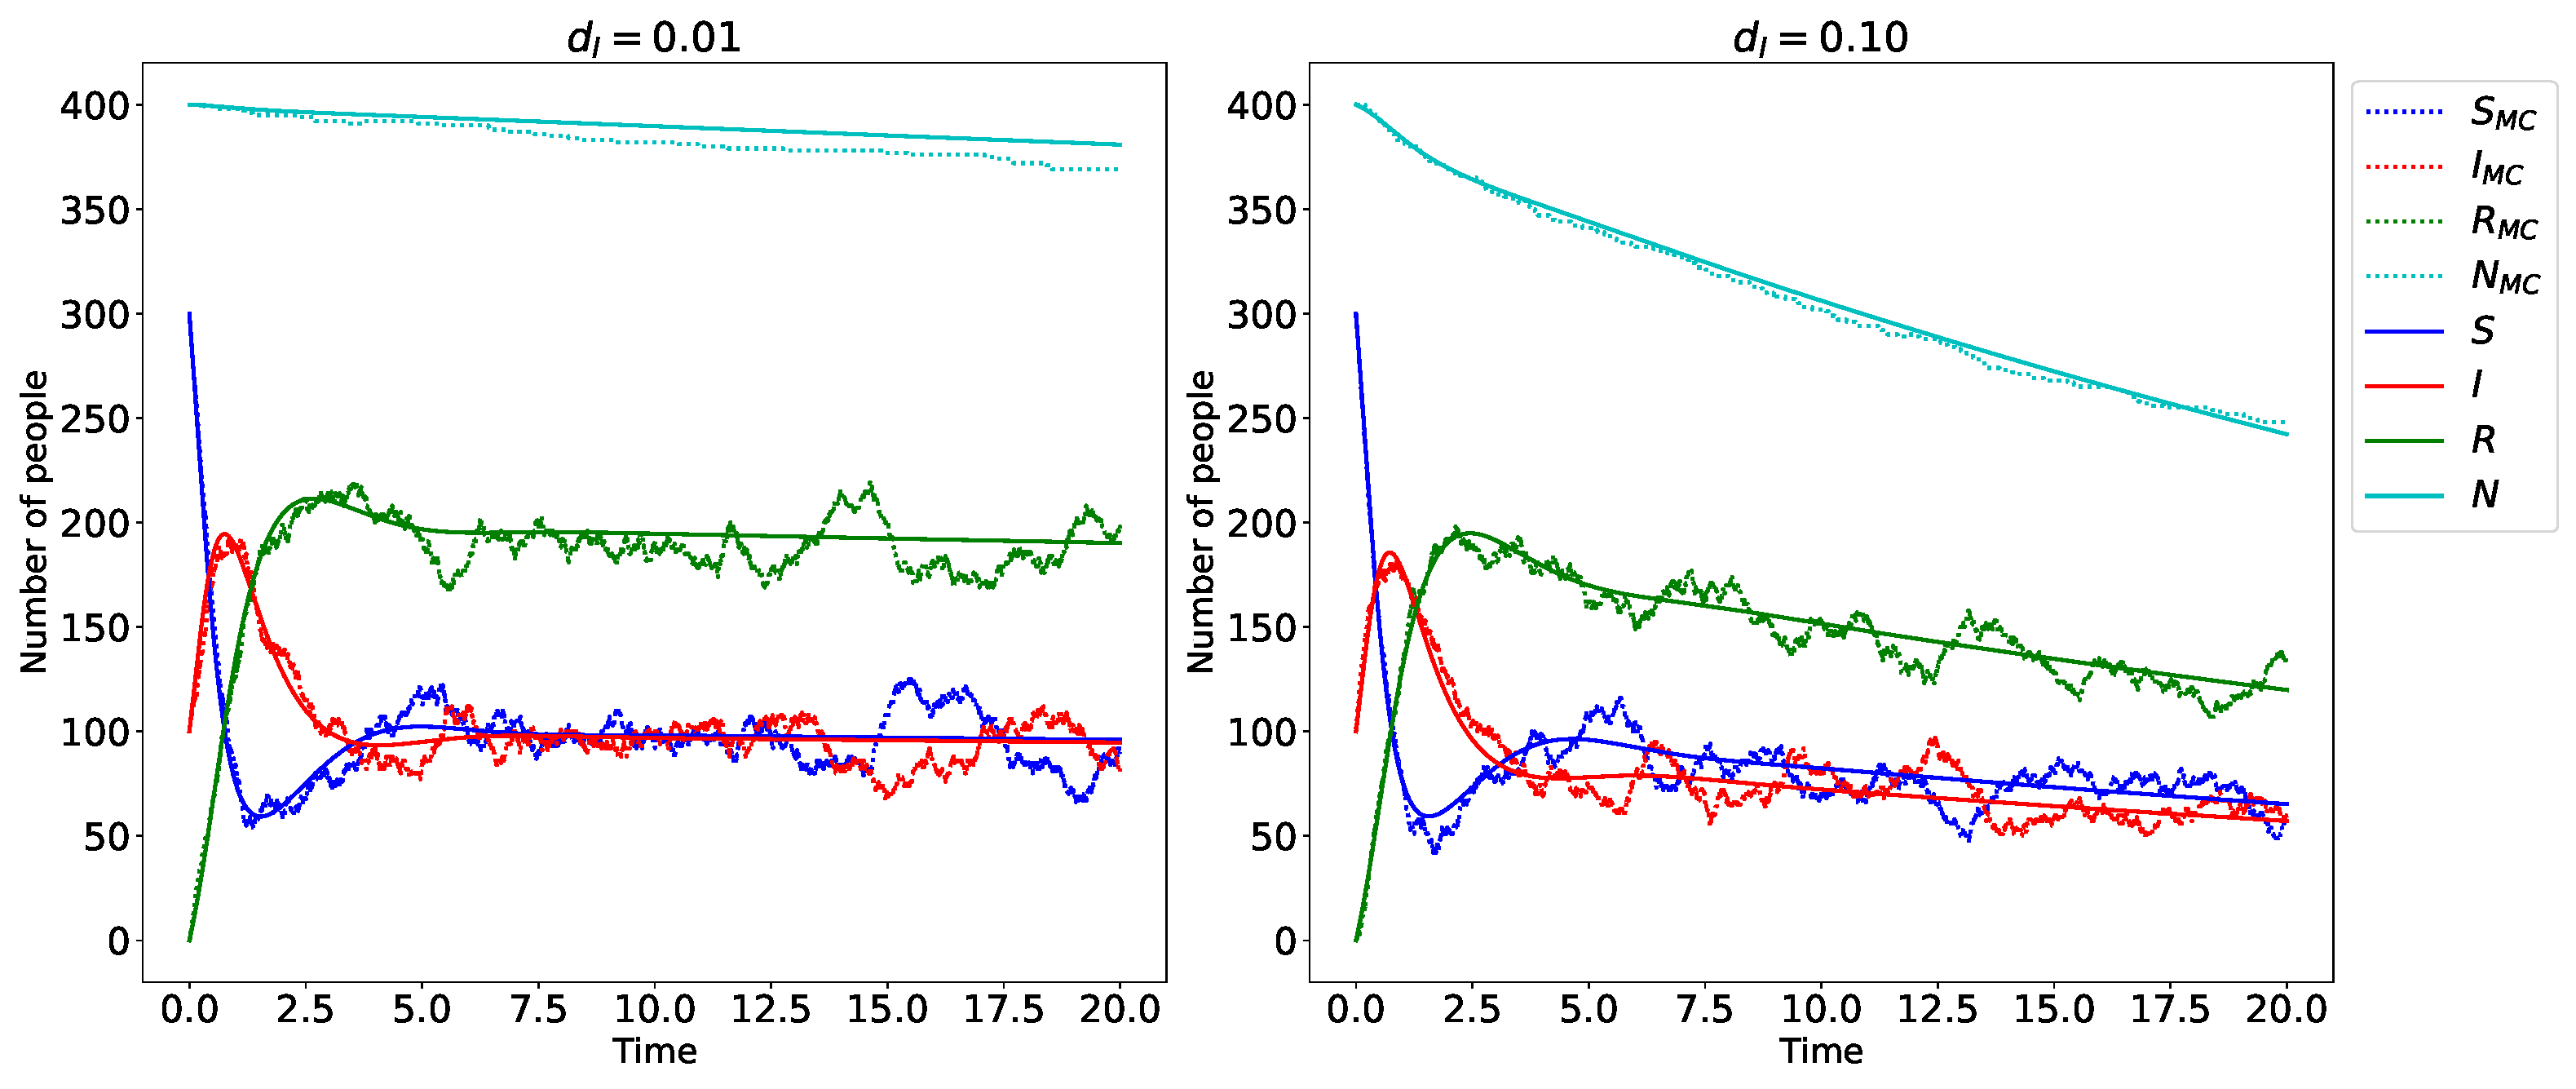
\includegraphics[width=\textwidth]{../figures/rk4_vs_mc_vd.pdf}
\caption{Monte Carlo and RK4 simulations of SIRS model with vital dynamics for varying $d_I$. $b = 1$, $d = 0.0003$ and $e = 0.0005$ for both populations. $N$ is the total population.}
\label{fig:mc:vital}
\end{figure}



\subsection{SIRS model with seasonal variation}
\iffalse
\begin{figure}[htb!]
    \centering
    \begin{subfigure}[b]{0.475\textwidth}
    \centering
    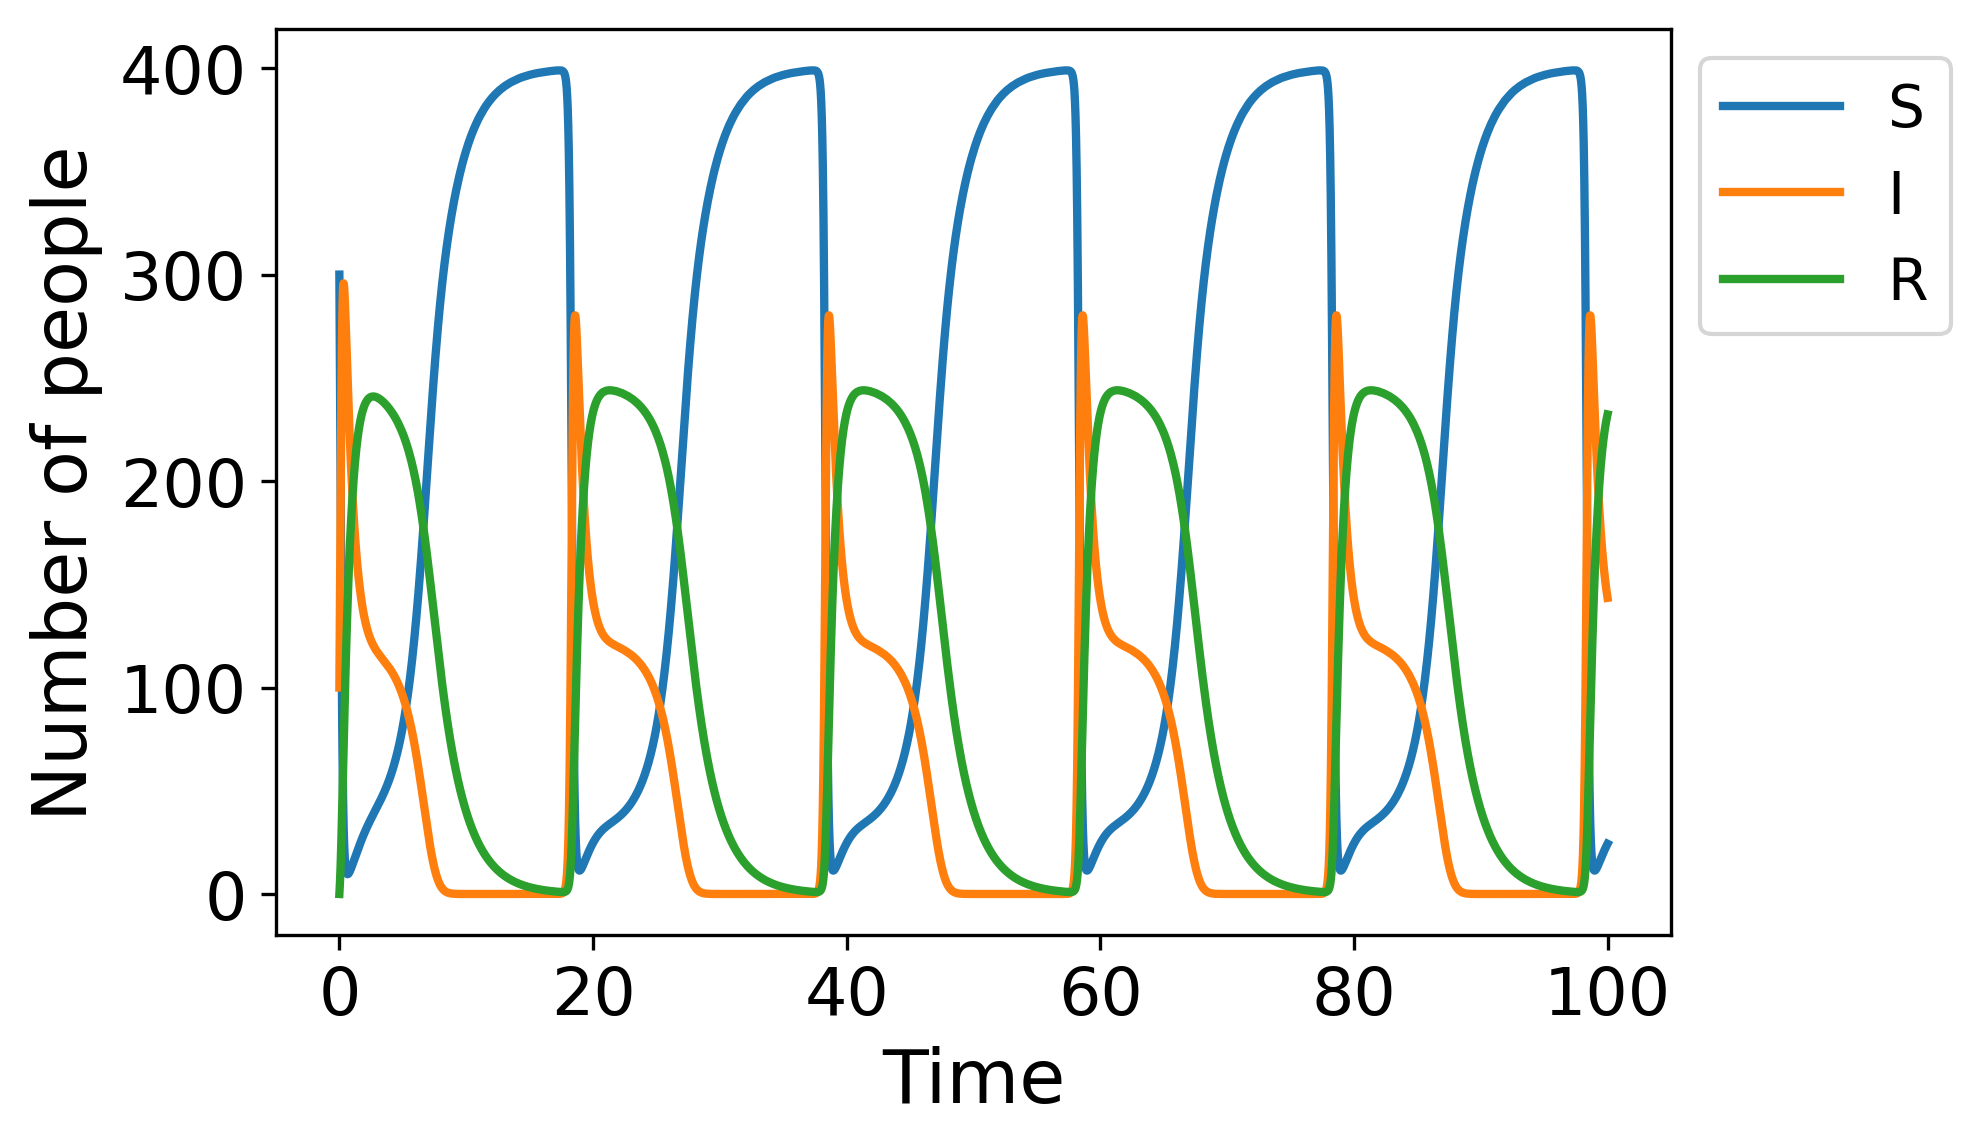
\includegraphics[width=0.9\textwidth]{../figures/SIRS_harmonical_rk4_b=1.png}
    \caption{}
    \label{fig:seasonal_b=1}
    \end{subfigure}
    \quad
    \begin{subfigure}[b]{0.475\textwidth}
    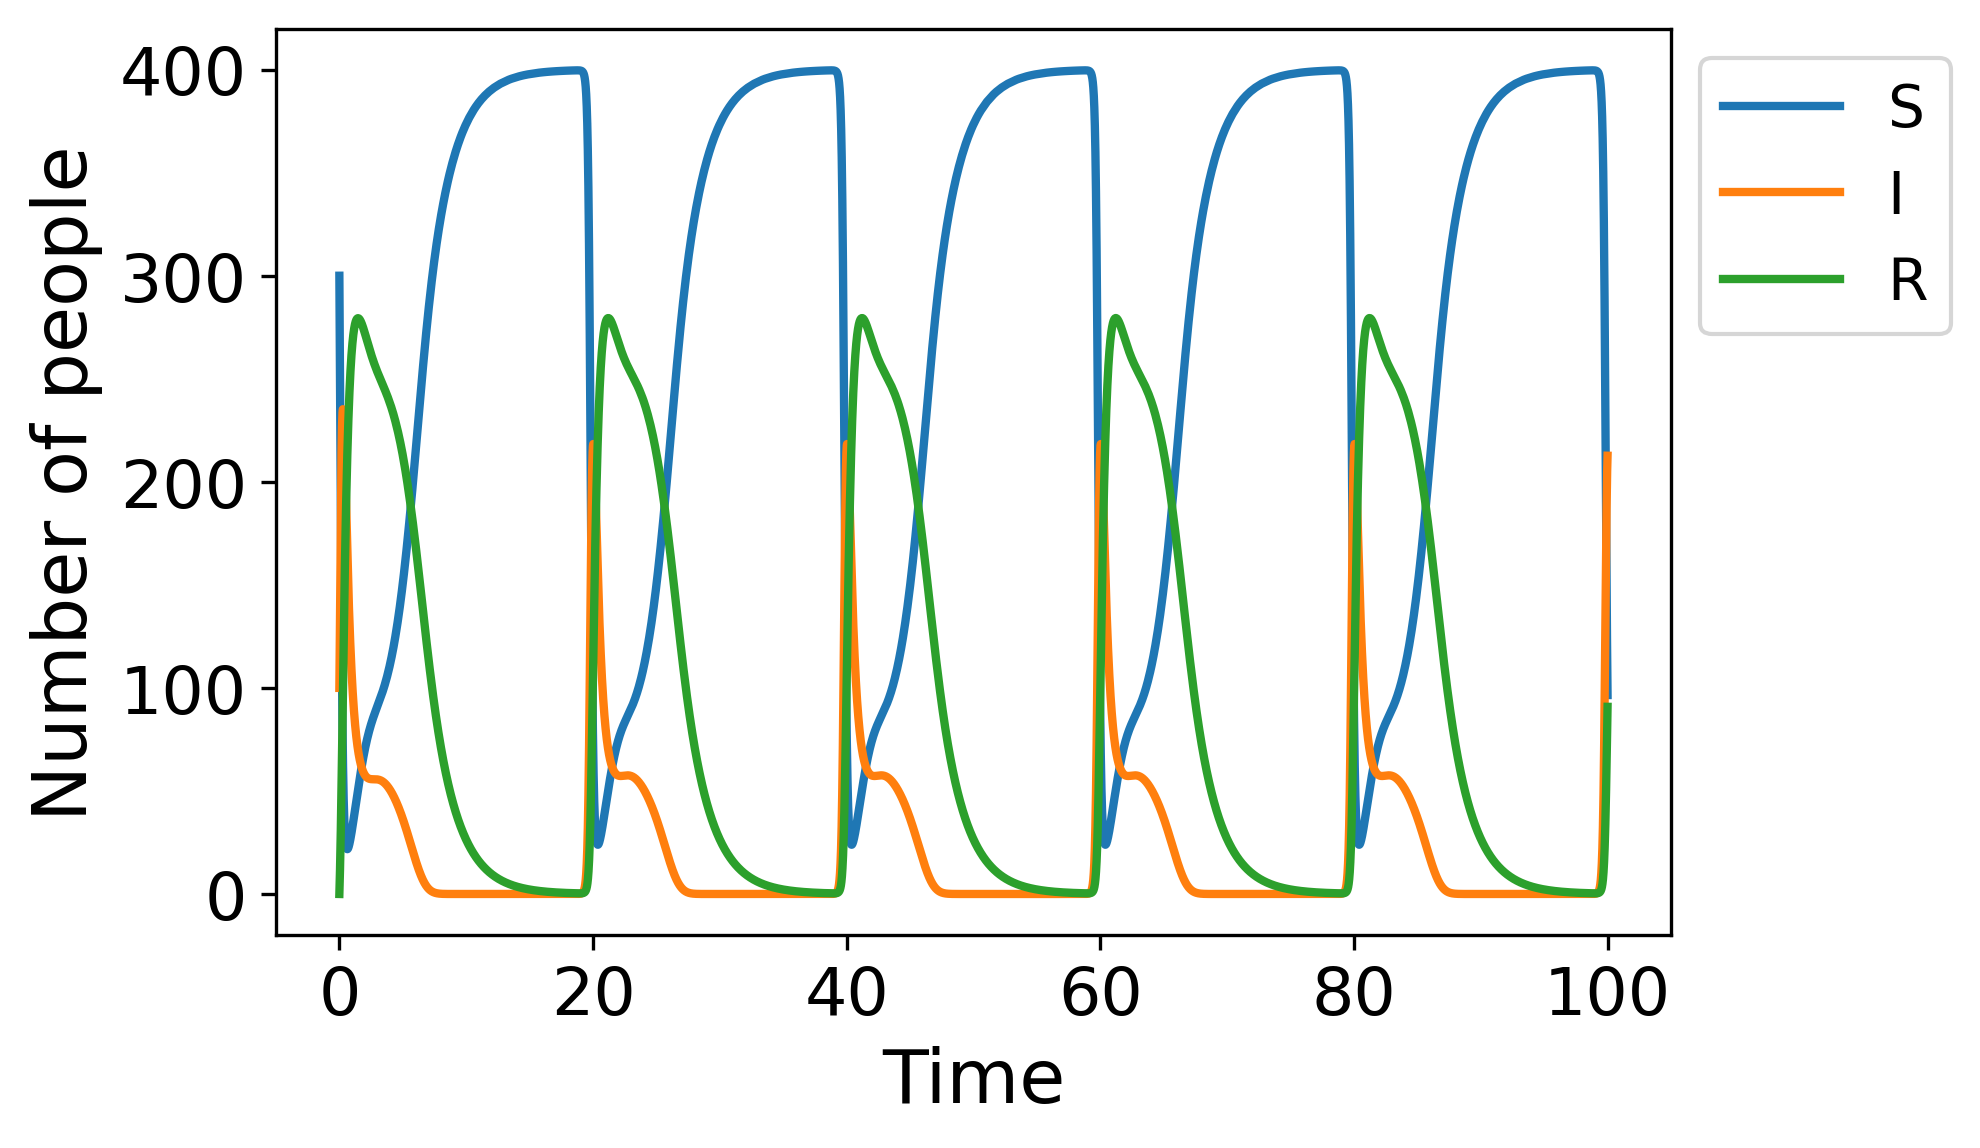
\includegraphics[width=0.9\textwidth]{../figures/SIRS_harmonical_rk4_b=2.png}
    \caption{}
    \label{fig:seasonal_b=2}
    \end{subfigure}
    
    \begin{subfigure}[b]{0.475\textwidth}
    \centering
    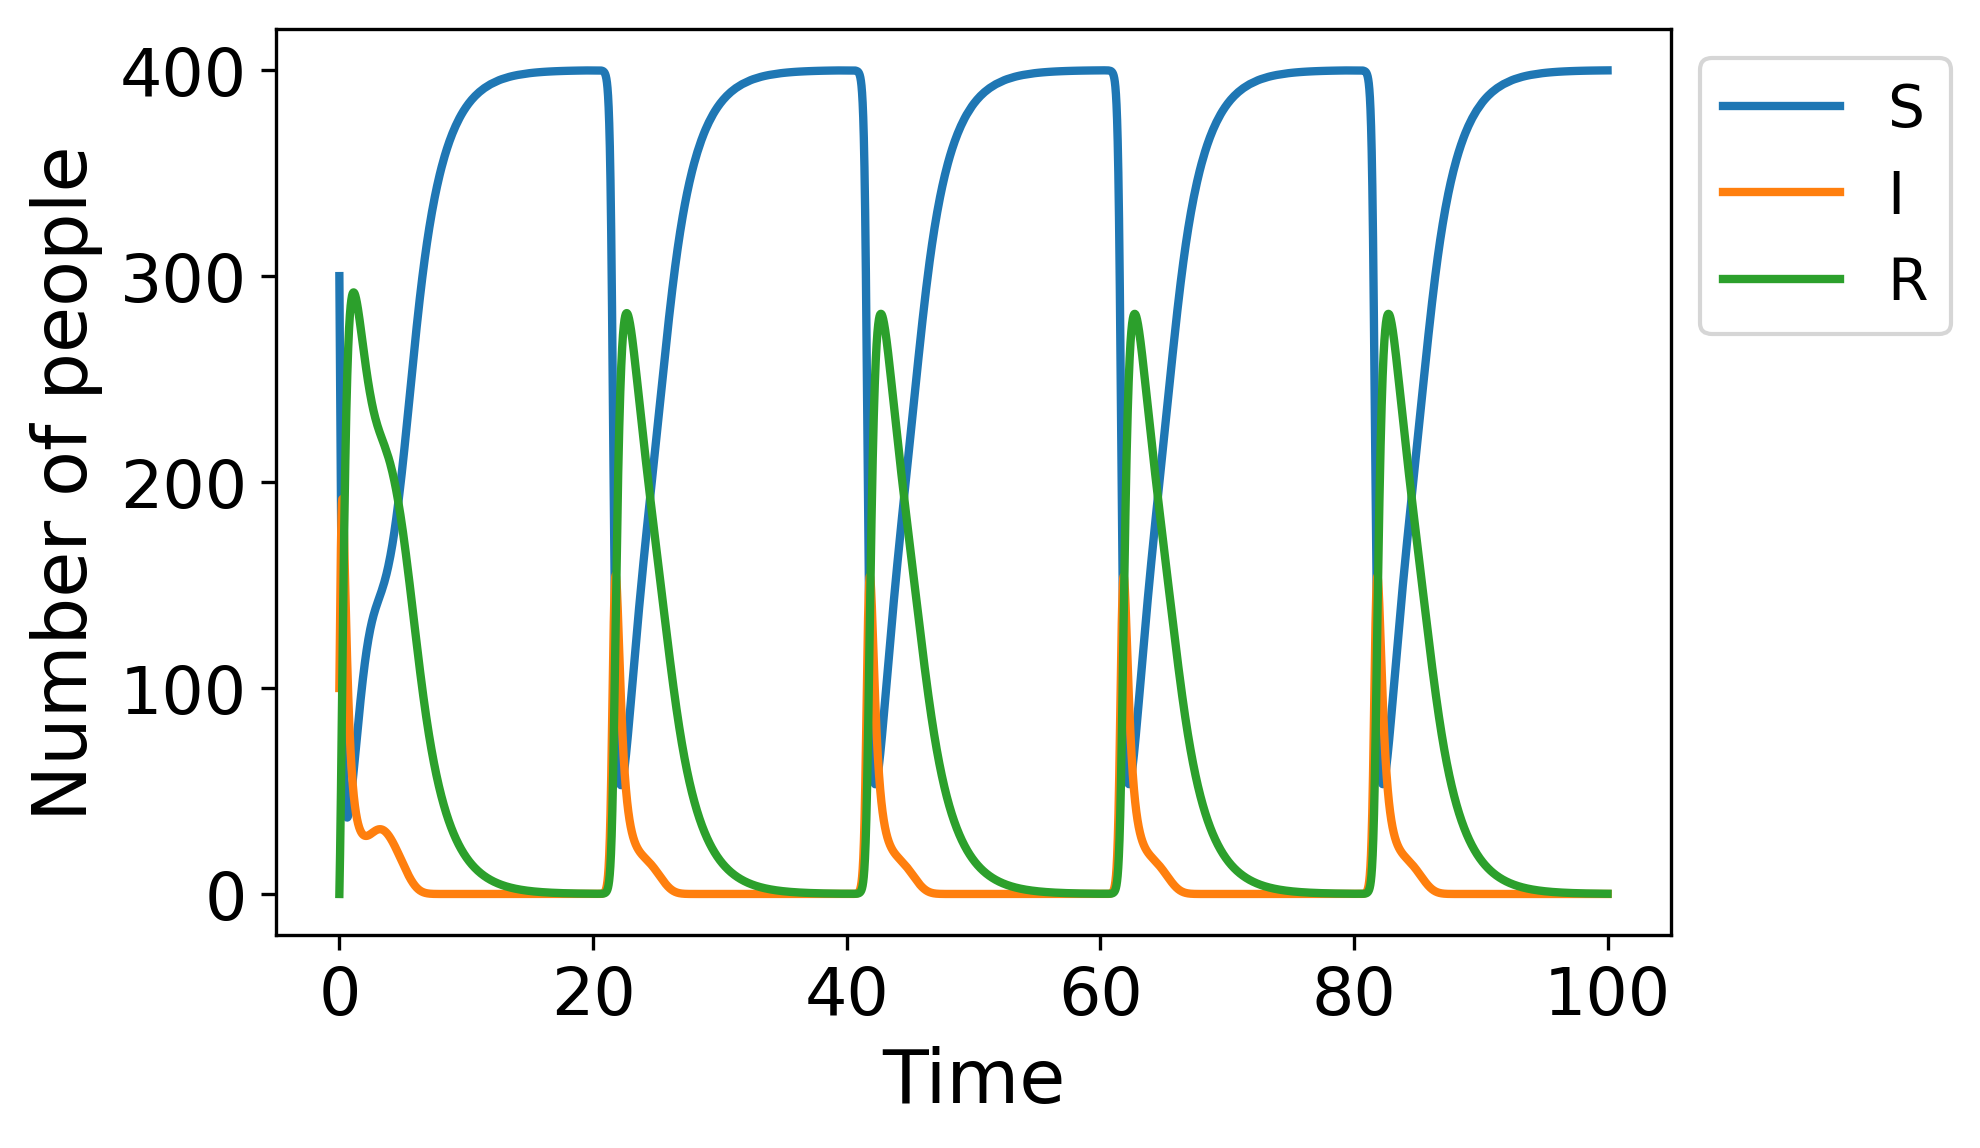
\includegraphics[width=0.9\textwidth]{../figures/SIRS_harmonical_rk4_b=3.png}
    \caption{}
    \label{fig:seasonal_b=3}
    \end{subfigure}
    \quad
    \begin{subfigure}[b]{0.475\textwidth}
    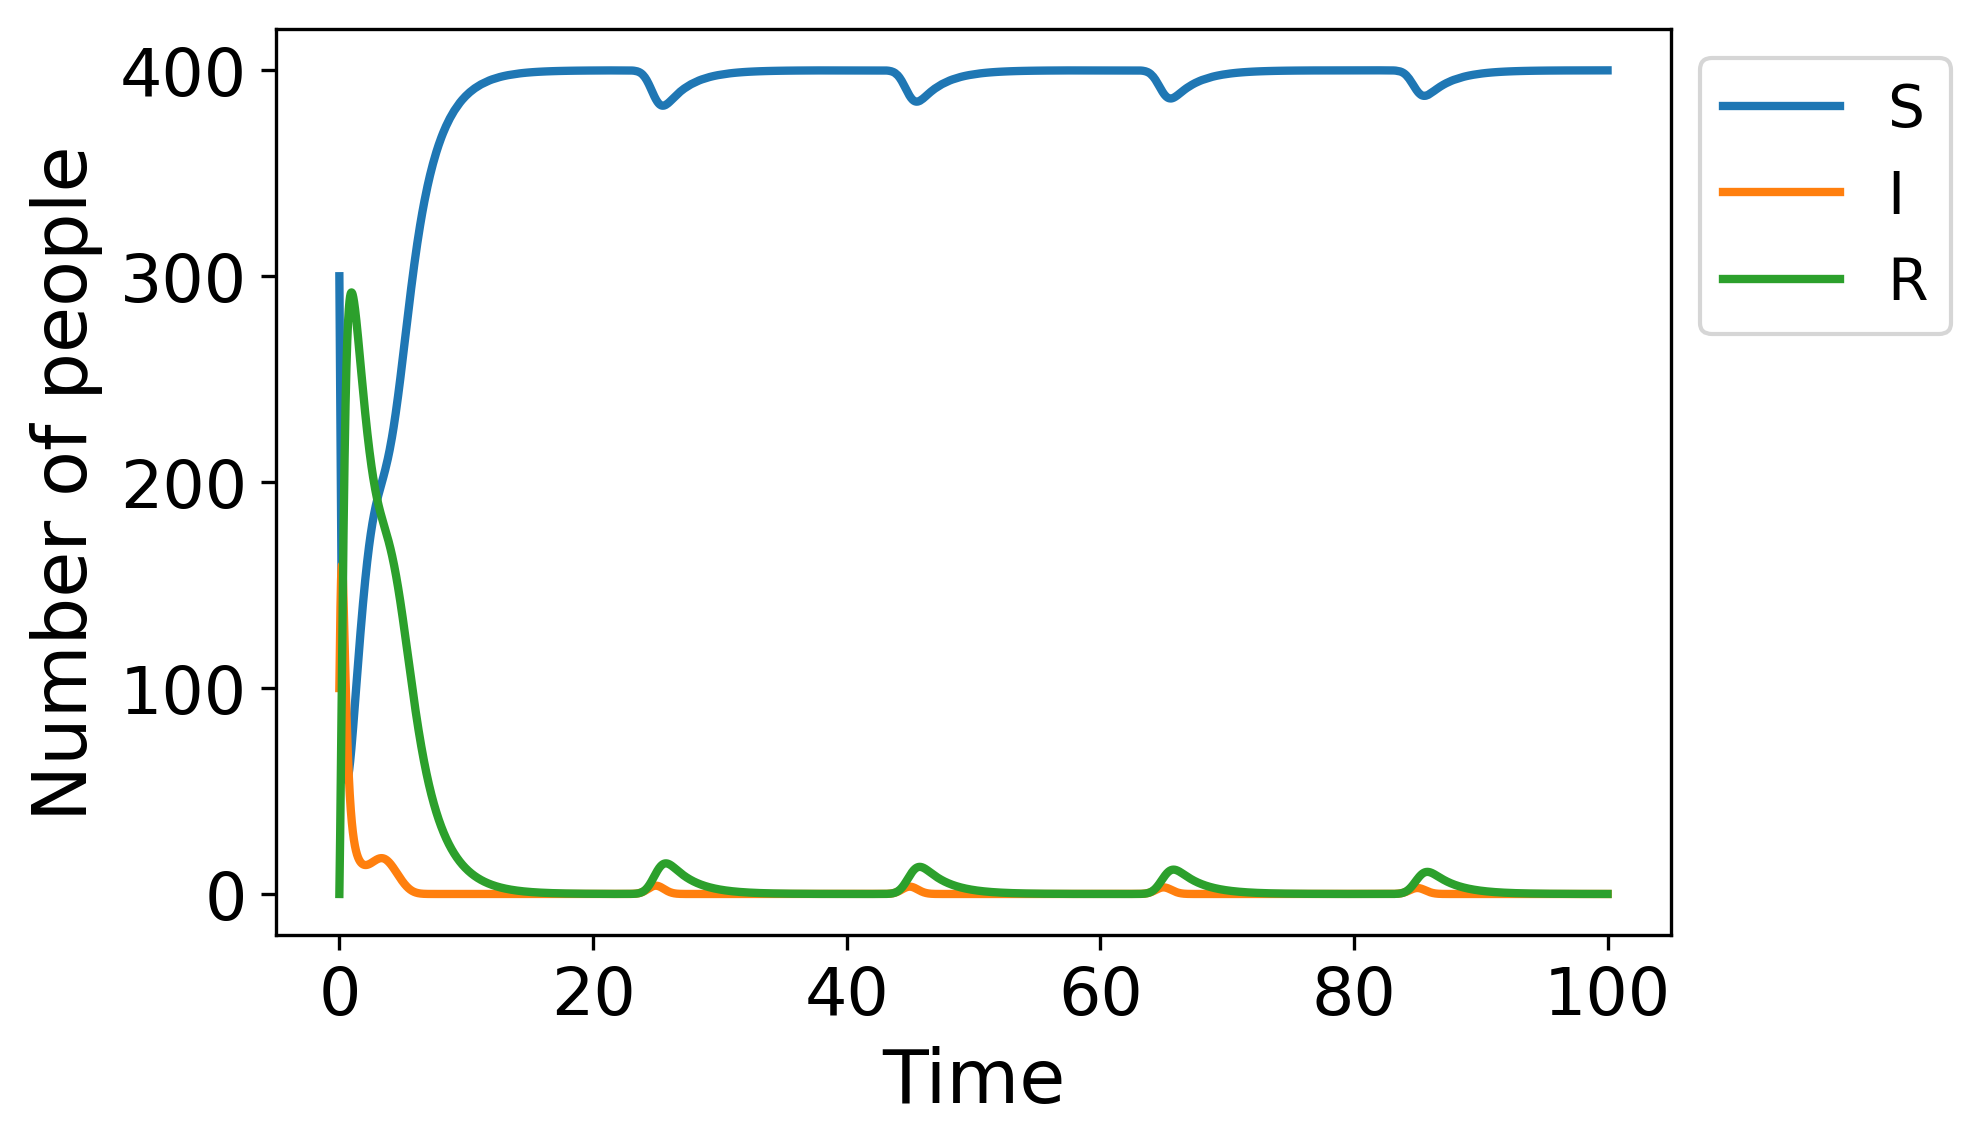
\includegraphics[width=0.9\textwidth]{../figures/SIRS_harmonical_rk4_b=4.png}
    \caption{}
    \label{fig:seasonal_b=4}
    \end{subfigure}
    \caption{The numerical solution of the SIRS model with seasonal variations using the fourth-order Runge-Kutta method with $N=400$, $I(0)=100$, $a=4$, $c=0.5$, $A=2.0$, $\omega=0.05\cdot2\pi$ fixed and the comparison of $S$, $I$, $R$ for (a)  $b=1$, (b) $b=2$, (c) $b=3$ and (d) $b=4$.}
    \label{fig:SIRS_rk4_seasonal}
\end{figure}
\fi

We now look at the effect of adding a cyclic function dependent on time $t$ that governs the rate of transmission $a = a(t)$ as described in equation (\ref{eq:a}).  

\begin{figure}[!htb]
\centering
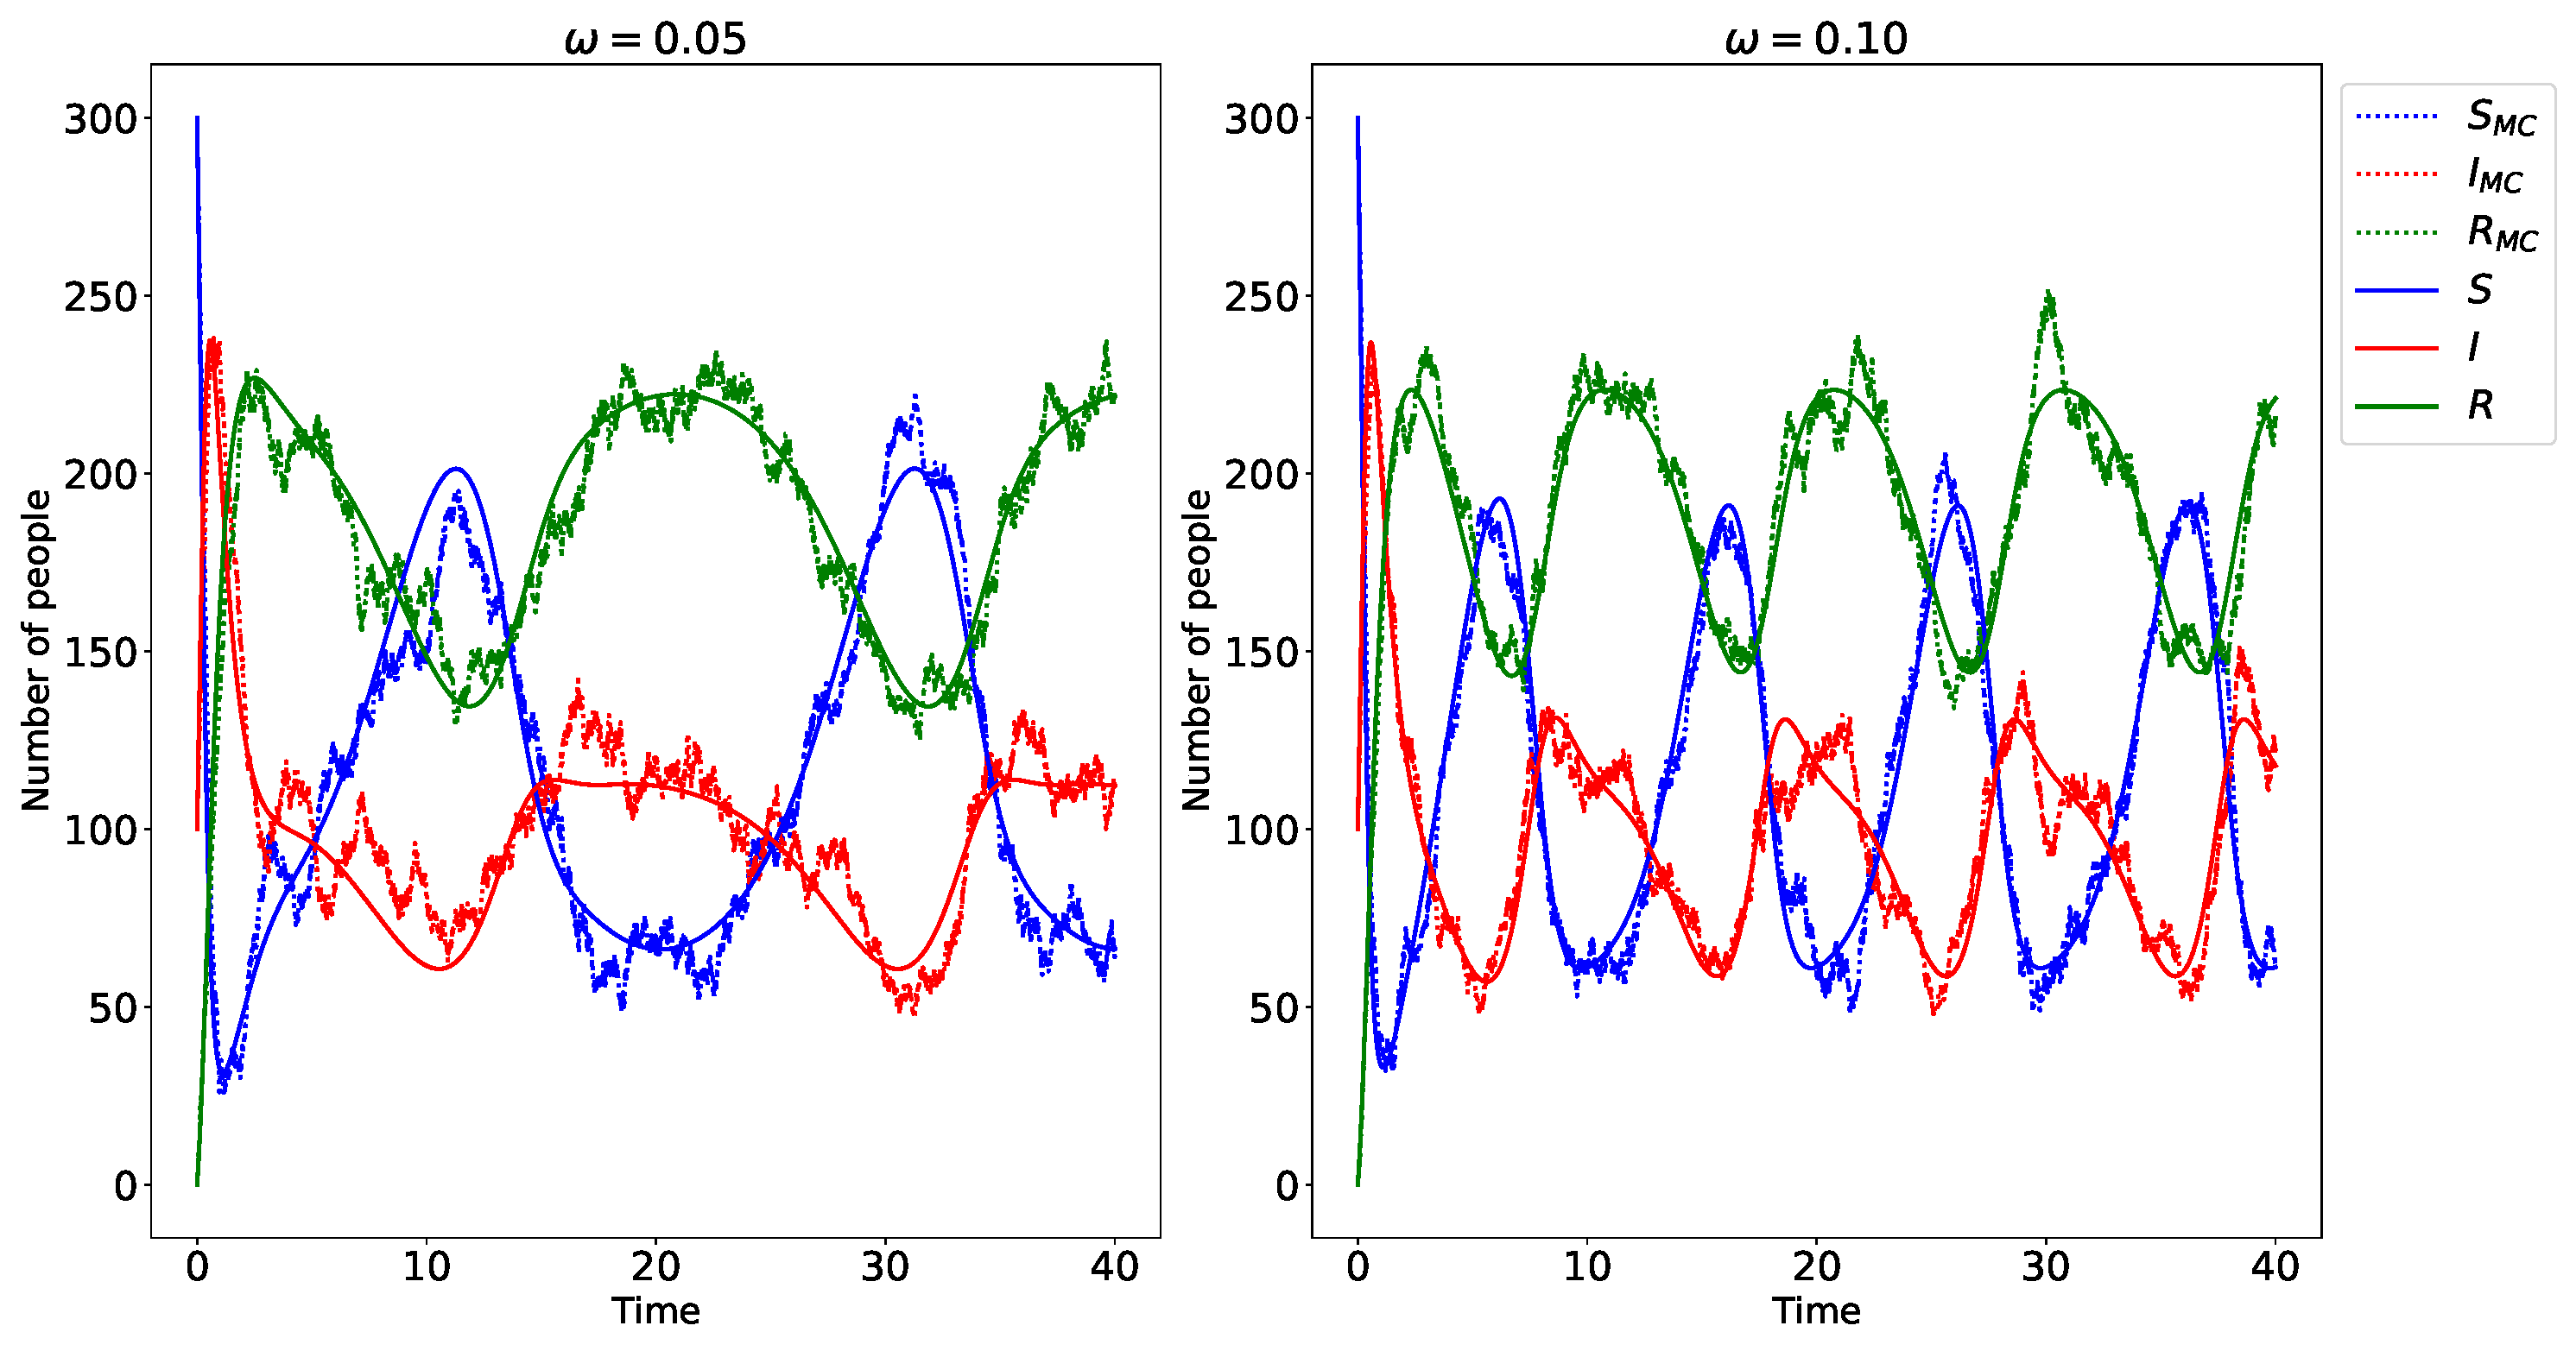
\includegraphics[width=\textwidth]{../figures/rk4_vs_mc_sv.pdf}
\caption{Monte Carlo and RK4 simulations of SIRS model with seasonal variation on the rate of transmission for varying $w$. $A = 2$ for both populations.}
\label{fig:mc:seasonal}
\end{figure}


\subsection{Vaccination}
Finally, we want to see how the addition of a vaccine would impact the spread of a disease, and the recovery of the population. Here we are using the linear function $f$ as described by equation (\ref{eq:f}).

\begin{figure}[!htb]
\centering
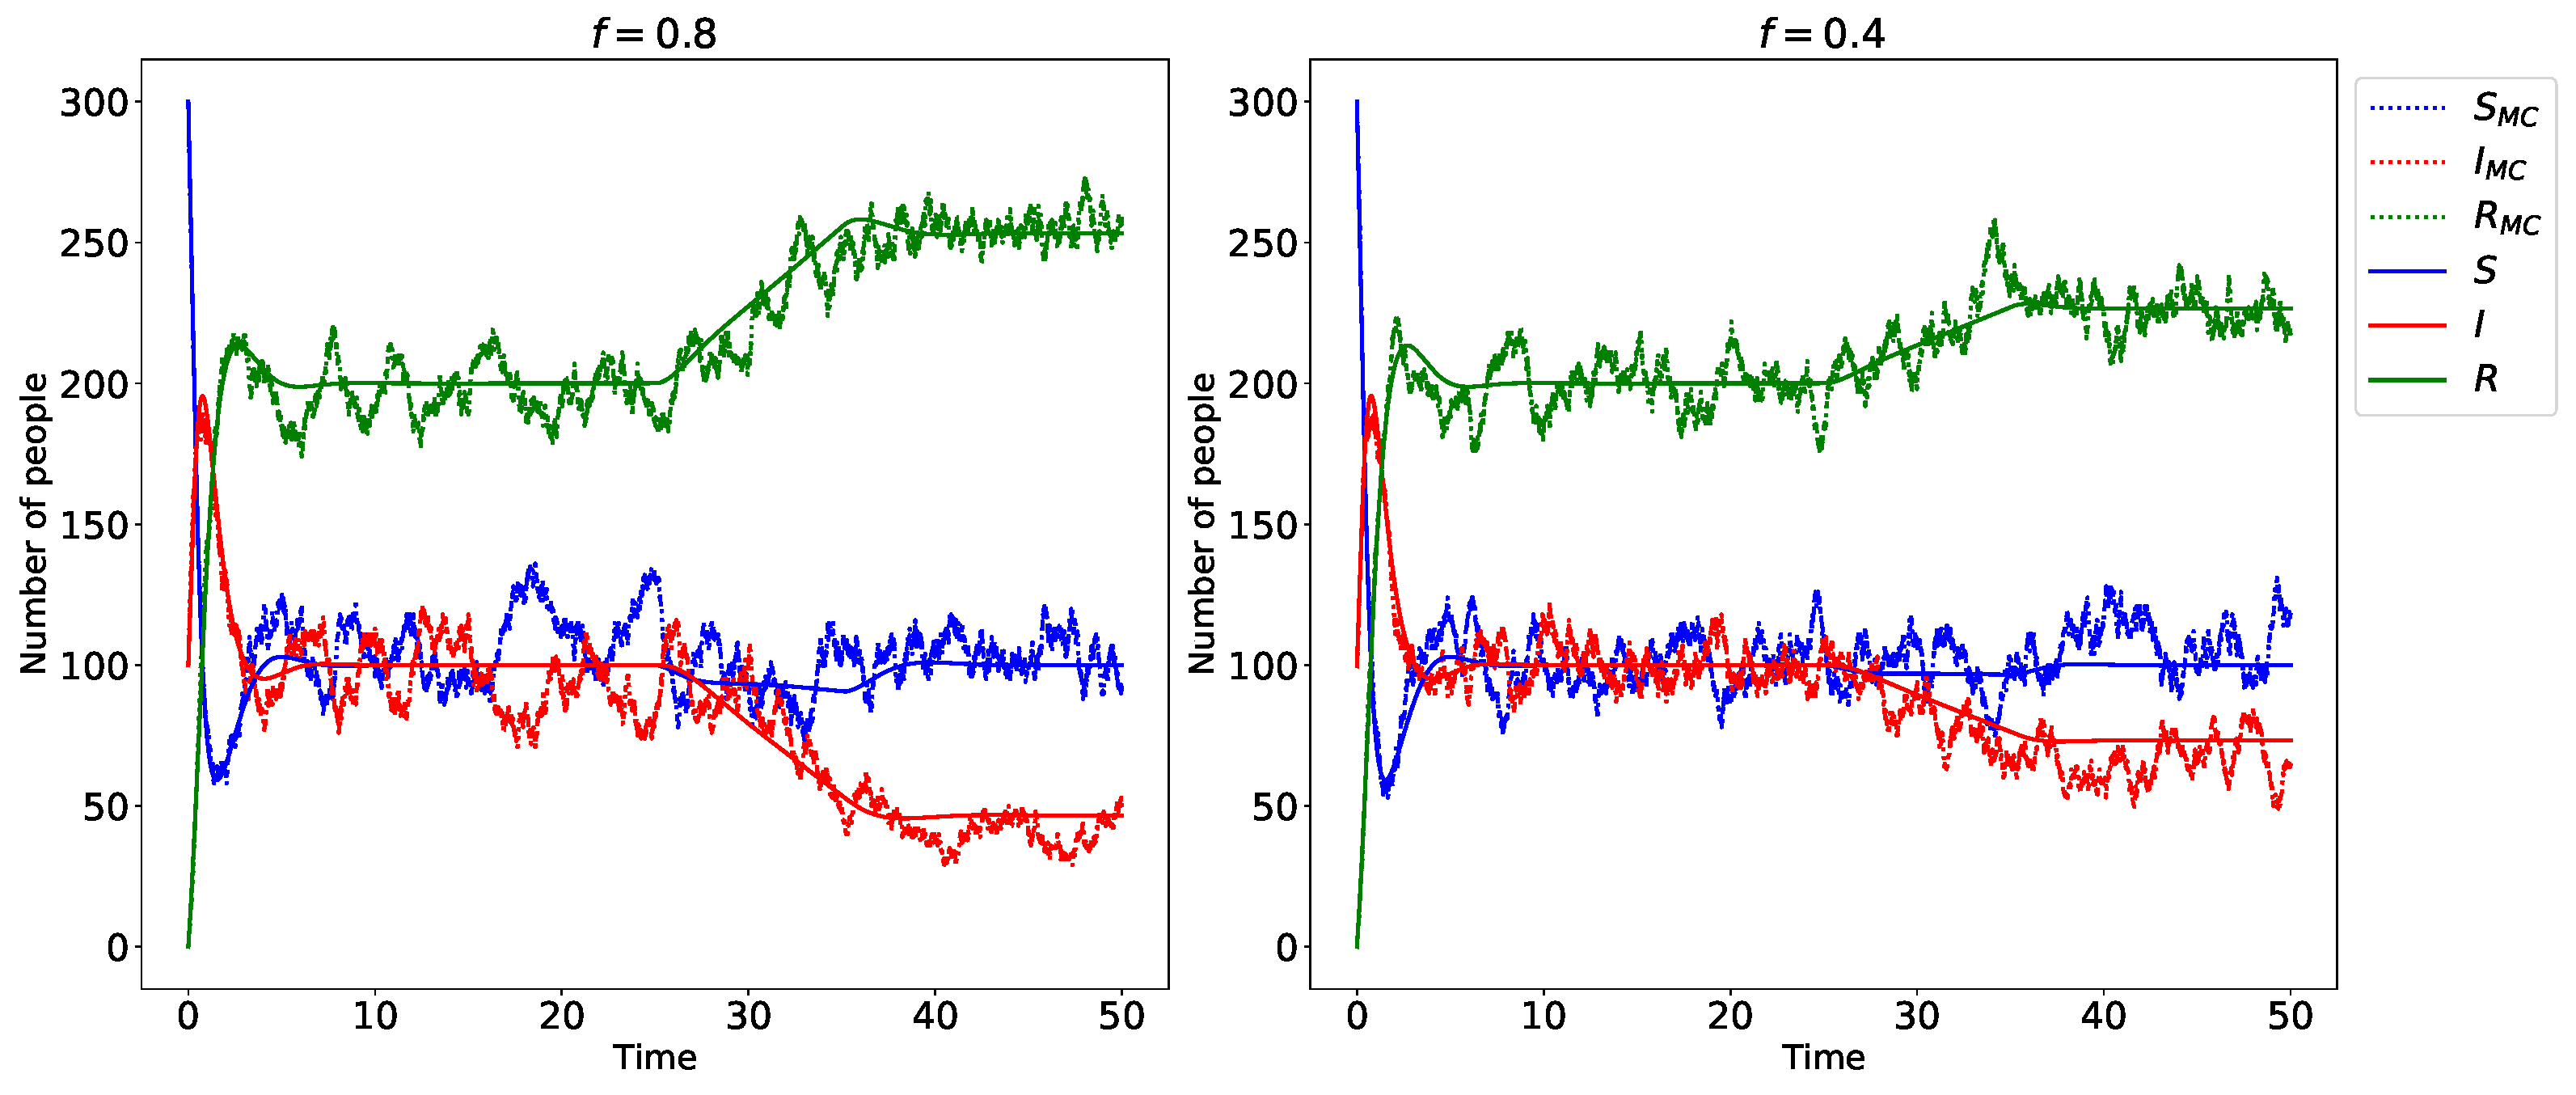
\includegraphics[width=\textwidth]{../figures/rk4_vs_mc_f.pdf}
\caption{A comparison of SIRS model with added vaccination parameter $f$, using both RK4 and MC simulation. Vaccination starts at $f_t = 25$}
\label{fig:mc:vaccine}
\end{figure}










\end{document}
